\documentclass[1p]{elsarticle_modified}
%\bibliographystyle{elsarticle-num}

%\usepackage[colorlinks]{hyperref}
%\usepackage{abbrmath_seonhwa} %\Abb, \Ascr, \Acal ,\Abf, \Afrak
\usepackage{amsfonts}
\usepackage{amssymb}
\usepackage{amsmath}
\usepackage{amsthm}
\usepackage{scalefnt}
\usepackage{amsbsy}
\usepackage{kotex}
\usepackage{caption}
\usepackage{subfig}
\usepackage{color}
\usepackage{graphicx}
\usepackage{xcolor} %% white, black, red, green, blue, cyan, magenta, yellow
\usepackage{float}
\usepackage{setspace}
\usepackage{hyperref}

\usepackage{tikz}
\usetikzlibrary{arrows}

\usepackage{multirow}
\usepackage{array} % fixed length table
\usepackage{hhline}

%%%%%%%%%%%%%%%%%%%%%
\makeatletter
\renewcommand*\env@matrix[1][\arraystretch]{%
	\edef\arraystretch{#1}%
	\hskip -\arraycolsep
	\let\@ifnextchar\new@ifnextchar
	\array{*\c@MaxMatrixCols c}}
\makeatother %https://tex.stackexchange.com/questions/14071/how-can-i-increase-the-line-spacing-in-a-matrix
%%%%%%%%%%%%%%%

\usepackage[normalem]{ulem}

\newcommand{\msout}[1]{\ifmmode\text{\sout{\ensuremath{#1}}}\else\sout{#1}\fi}
%SOURCE: \msout is \stkout macro in https://tex.stackexchange.com/questions/20609/strikeout-in-math-mode

\newcommand{\cancel}[1]{
	\ifmmode
	{\color{red}\msout{#1}}
	\else
	{\color{red}\sout{#1}}
	\fi
}

\newcommand{\add}[1]{
	{\color{blue}\uwave{#1}}
}

\newcommand{\replace}[2]{
	\ifmmode
	{\color{red}\msout{#1}}{\color{blue}\uwave{#2}}
	\else
	{\color{red}\sout{#1}}{\color{blue}\uwave{#2}}
	\fi
}

\newcommand{\Sol}{\mathcal{S}} %segment
\newcommand{\D}{D} %diagram
\newcommand{\A}{\mathcal{A}} %arc


%%%%%%%%%%%%%%%%%%%%%%%%%%%%%5 test

\def\sl{\operatorname{\textup{SL}}(2,\Cbb)}
\def\psl{\operatorname{\textup{PSL}}(2,\Cbb)}
\def\quan{\mkern 1mu \triangleright \mkern 1mu}

\theoremstyle{definition}
\newtheorem{thm}{Theorem}[section]
\newtheorem{prop}[thm]{Proposition}
\newtheorem{lem}[thm]{Lemma}
\newtheorem{ques}[thm]{Question}
\newtheorem{cor}[thm]{Corollary}
\newtheorem{defn}[thm]{Definition}
\newtheorem{exam}[thm]{Example}
\newtheorem{rmk}[thm]{Remark}
\newtheorem{alg}[thm]{Algorithm}

\newcommand{\I}{\sqrt{-1}}
\begin{document}

%\begin{frontmatter}
%
%\title{Boundary parabolic representations of knots up to 8 crossings}
%
%%% Group authors per affiliation:
%\author{Yunhi Cho} 
%\address{Department of Mathematics, University of Seoul, Seoul, Korea}
%\ead{yhcho@uos.ac.kr}
%
%
%\author{Seonhwa Kim} %\fnref{s_kim}}
%\address{Center for Geometry and Physics, Institute for Basic Science, Pohang, 37673, Korea}
%\ead{ryeona17@ibs.re.kr}
%
%\author{Hyuk Kim}
%\address{Department of Mathematical Sciences, Seoul National University, Seoul 08826, Korea}
%\ead{hyukkim@snu.ac.kr}
%
%\author{Seokbeom Yoon}
%\address{Department of Mathematical Sciences, Seoul National University, Seoul, 08826,  Korea}
%\ead{sbyoon15@snu.ac.kr}
%
%\begin{abstract}
%We find all boundary parabolic representation of knots up to 8 crossings.
%
%\end{abstract}
%\begin{keyword}
%    \MSC[2010] 57M25 
%\end{keyword}
%
%\end{frontmatter}

%\linenumbers
%\tableofcontents
%
\newcommand\colored[1]{\textcolor{white}{\rule[-0.35ex]{0.8em}{1.4ex}}\kern-0.8em\color{red} #1}%
%\newcommand\colored[1]{\textcolor{white}{ #1}\kern-2.17ex	\textcolor{white}{ #1}\kern-1.81ex	\textcolor{white}{ #1}\kern-2.15ex\color{red}#1	}

{\Large $\underline{12a_{0962}~(K12a_{0962})}$}

\setlength{\tabcolsep}{10pt}
\renewcommand{\arraystretch}{1.6}
\vspace{1cm}\begin{tabular}{m{100pt}>{\centering\arraybackslash}m{274pt}}
\multirow{5}{120pt}{
	\centering
	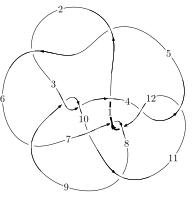
\includegraphics[width=112pt]{../../../GIT/diagram.site/Diagrams/png/1763_12a_0962.png}\\
\ \ \ A knot diagram\footnotemark}&
\allowdisplaybreaks
\textbf{Linearized knot diagam} \\
\cline{2-2}
 &
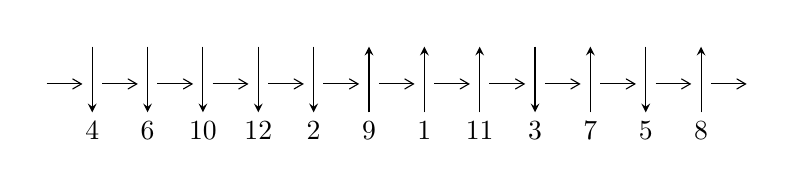
\begin{tikzpicture}[x=20pt, y=17pt]
	% nodes
	\node (C0) at (0, 0) {};
	\node (C1) at (1, 0) {};
	\node (C1U) at (1, +1) {};
	\node (C1D) at (1, -1) {4};

	\node (C2) at (2, 0) {};
	\node (C2U) at (2, +1) {};
	\node (C2D) at (2, -1) {6};

	\node (C3) at (3, 0) {};
	\node (C3U) at (3, +1) {};
	\node (C3D) at (3, -1) {10};

	\node (C4) at (4, 0) {};
	\node (C4U) at (4, +1) {};
	\node (C4D) at (4, -1) {12};

	\node (C5) at (5, 0) {};
	\node (C5U) at (5, +1) {};
	\node (C5D) at (5, -1) {2};

	\node (C6) at (6, 0) {};
	\node (C6U) at (6, +1) {};
	\node (C6D) at (6, -1) {9};

	\node (C7) at (7, 0) {};
	\node (C7U) at (7, +1) {};
	\node (C7D) at (7, -1) {1};

	\node (C8) at (8, 0) {};
	\node (C8U) at (8, +1) {};
	\node (C8D) at (8, -1) {11};

	\node (C9) at (9, 0) {};
	\node (C9U) at (9, +1) {};
	\node (C9D) at (9, -1) {3};

	\node (C10) at (10, 0) {};
	\node (C10U) at (10, +1) {};
	\node (C10D) at (10, -1) {7};

	\node (C11) at (11, 0) {};
	\node (C11U) at (11, +1) {};
	\node (C11D) at (11, -1) {5};

	\node (C12) at (12, 0) {};
	\node (C12U) at (12, +1) {};
	\node (C12D) at (12, -1) {8};
	\node (C13) at (13, 0) {};

	% arrows
	\draw[->,>={angle 60}]
	(C0) edge (C1) (C1) edge (C2) (C2) edge (C3) (C3) edge (C4) (C4) edge (C5) (C5) edge (C6) (C6) edge (C7) (C7) edge (C8) (C8) edge (C9) (C9) edge (C10) (C10) edge (C11) (C11) edge (C12) (C12) edge (C13) ;	\draw[->,>=stealth]
	(C1U) edge (C1D) (C2U) edge (C2D) (C3U) edge (C3D) (C4U) edge (C4D) (C5U) edge (C5D) (C6D) edge (C6U) (C7D) edge (C7U) (C8D) edge (C8U) (C9U) edge (C9D) (C10D) edge (C10U) (C11U) edge (C11D) (C12D) edge (C12U) ;
	\end{tikzpicture} \\
\hhline{~~} \\& 
\textbf{Solving Sequence} \\ \cline{2-2} 
 &
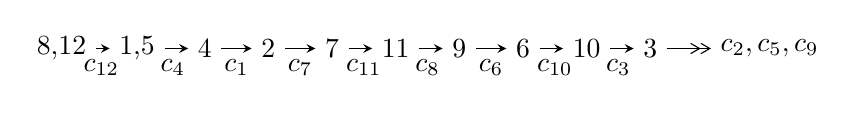
\begin{tikzpicture}[x=23pt, y=7pt]
	% node
	\node (A0) at (-1/8, 0) {8,12};
	\node (A1) at (17/16, 0) {1,5};
	\node (A2) at (17/8, 0) {4};
	\node (A3) at (25/8, 0) {2};
	\node (A4) at (33/8, 0) {7};
	\node (A5) at (41/8, 0) {11};
	\node (A6) at (49/8, 0) {9};
	\node (A7) at (57/8, 0) {6};
	\node (A8) at (65/8, 0) {10};
	\node (A9) at (73/8, 0) {3};
	\node (C1) at (1/2, -1) {$c_{12}$};
	\node (C2) at (13/8, -1) {$c_{4}$};
	\node (C3) at (21/8, -1) {$c_{1}$};
	\node (C4) at (29/8, -1) {$c_{7}$};
	\node (C5) at (37/8, -1) {$c_{11}$};
	\node (C6) at (45/8, -1) {$c_{8}$};
	\node (C7) at (53/8, -1) {$c_{6}$};
	\node (C8) at (61/8, -1) {$c_{10}$};
	\node (C9) at (69/8, -1) {$c_{3}$};
	\node (A10) at (11, 0) {$c_{2},c_{5},c_{9}$};

	% edge
	\draw[->,>=stealth]	
	(A0) edge (A1) (A1) edge (A2) (A2) edge (A3) (A3) edge (A4) (A4) edge (A5) (A5) edge (A6) (A6) edge (A7) (A7) edge (A8) (A8) edge (A9) ;
	\draw[->>,>={angle 60}]	
	(A9) edge (A10);
\end{tikzpicture} \\ 

\end{tabular} \\

\footnotetext{
The image of knot diagram is generated by the software ``\textbf{Draw programme}" developed by Andrew Bartholomew(\url{http://www.layer8.co.uk/maths/draw/index.htm\#Running-draw}), where we modified some parts for our purpose(\url{https://github.com/CATsTAILs/LinksPainter}).
}\phantom \\ \newline 
\centering \textbf{Ideals for irreducible components\footnotemark of $X_{\text{par}}$} 
 
\begin{align*}
I^u_{1}&=\langle 
-1.47858\times10^{906} u^{167}-1.86588\times10^{906} u^{166}+\cdots+2.81415\times10^{907} b-2.43977\times10^{910},\\
\phantom{I^u_{1}}&\phantom{= \langle  }-9.74692\times10^{910} u^{167}-1.64355\times10^{911} u^{166}+\cdots+3.51515\times10^{911} a-7.67366\times10^{914},\\
\phantom{I^u_{1}}&\phantom{= \langle  }u^{168}+2 u^{167}+\cdots+5047 u-12491\rangle \\
I^u_{2}&=\langle 
2.04586\times10^{50} u^{48}+1.66191\times10^{50} u^{47}+\cdots+1.22185\times10^{49} b+6.36745\times10^{50},\\
\phantom{I^u_{2}}&\phantom{= \langle  }2.72498\times10^{51} u^{48}+1.13526\times10^{51} u^{47}+\cdots+8.55296\times10^{49} a+3.50591\times10^{52},\;u^{49}+u^{48}+\cdots-19 u-7\rangle \\
\\
\end{align*}
\raggedright * 2 irreducible components of $\dim_{\mathbb{C}}=0$, with total 217 representations.\\
\footnotetext{All coefficients of polynomials are rational numbers. But the coefficients are sometimes approximated in decimal forms when there is not enough margin.}
\newpage
\renewcommand{\arraystretch}{1}
\centering \section*{I. $I^u_{1}= \langle -1.48\times10^{906} u^{167}-1.87\times10^{906} u^{166}+\cdots+2.81\times10^{907} b-2.44\times10^{910},\;-9.75\times10^{910} u^{167}-1.64\times10^{911} u^{166}+\cdots+3.52\times10^{911} a-7.67\times10^{914},\;u^{168}+2 u^{167}+\cdots+5047 u-12491 \rangle$}
\flushleft \textbf{(i) Arc colorings}\\
\begin{tabular}{m{7pt} m{180pt} m{7pt} m{180pt} }
\flushright $a_{8}=$&$\begin{pmatrix}0\\u\end{pmatrix}$ \\
\flushright $a_{12}=$&$\begin{pmatrix}1\\0\end{pmatrix}$ \\
\flushright $a_{1}=$&$\begin{pmatrix}1\\- u^2\end{pmatrix}$ \\
\flushright $a_{5}=$&$\begin{pmatrix}0.277283 u^{167}+0.467562 u^{166}+\cdots-7171.07 u+2183.02\\0.0525410 u^{167}+0.0663036 u^{166}+\cdots-1722.43 u+866.965\end{pmatrix}$ \\
\flushright $a_{4}=$&$\begin{pmatrix}0.329824 u^{167}+0.533866 u^{166}+\cdots-8893.50 u+3049.99\\0.0525410 u^{167}+0.0663036 u^{166}+\cdots-1722.43 u+866.965\end{pmatrix}$ \\
\flushright $a_{2}=$&$\begin{pmatrix}-0.474713 u^{167}-0.734990 u^{166}+\cdots+11669.8 u-5374.80\\0.0652619 u^{167}+0.172891 u^{166}+\cdots-691.352 u-949.598\end{pmatrix}$ \\
\flushright $a_{7}=$&$\begin{pmatrix}- u\\u^3+u\end{pmatrix}$ \\
\flushright $a_{11}=$&$\begin{pmatrix}0.182365 u^{167}+0.456811 u^{166}+\cdots-3559.96 u-1998.14\\0.0592164 u^{167}+0.164564 u^{166}+\cdots-1628.68 u-776.813\end{pmatrix}$ \\
\flushright $a_{9}=$&$\begin{pmatrix}0.209000 u^{167}+0.592035 u^{166}+\cdots-3261.57 u-3553.75\\-0.00209783 u^{167}-0.0814685 u^{166}+\cdots-172.095 u+1475.68\end{pmatrix}$ \\
\flushright $a_{6}=$&$\begin{pmatrix}-0.387045 u^{167}-0.716368 u^{166}+\cdots+8369.78 u-1384.09\\0.0874866 u^{167}+0.240025 u^{166}+\cdots-1771.47 u-1142.82\end{pmatrix}$ \\
\flushright $a_{10}=$&$\begin{pmatrix}0.248860 u^{167}+0.638379 u^{166}+\cdots-4901.42 u-2990.00\\0.0303659 u^{167}+0.0906564 u^{166}+\cdots-872.648 u-391.732\end{pmatrix}$ \\
\flushright $a_{3}=$&$\begin{pmatrix}0.342467 u^{167}+0.755504 u^{166}+\cdots-6879.19 u-1168.44\\0.0000903648 u^{167}-0.0687298 u^{166}+\cdots-923.769 u+1485.07\end{pmatrix}$\\&\end{tabular}
\flushleft \textbf{(ii) Obstruction class $= -1$}\\~\\
\flushleft \textbf{(iii) Cusp Shapes $= 0.114789 u^{167}+0.346935 u^{166}+\cdots-3505.02 u-4107.41$}\\~\\
\newpage\renewcommand{\arraystretch}{1}
\flushleft \textbf{(iv) u-Polynomials at the component}\newline \\
\begin{tabular}{m{50pt}|m{274pt}}
Crossings & \hspace{64pt}u-Polynomials at each crossing \\
\hline $$\begin{aligned}c_{1}\end{aligned}$$&$\begin{aligned}
&u^{168}-16 u^{167}+\cdots-7296363 u-2529737
\end{aligned}$\\
\hline $$\begin{aligned}c_{2},c_{5}\end{aligned}$$&$\begin{aligned}
&u^{168}+4 u^{167}+\cdots-16865158 u-846613
\end{aligned}$\\
\hline $$\begin{aligned}c_{3},c_{9}\end{aligned}$$&$\begin{aligned}
&u^{168}+u^{167}+\cdots-150117 u+83053
\end{aligned}$\\
\hline $$\begin{aligned}c_{4},c_{11}\end{aligned}$$&$\begin{aligned}
&u^{168}+2 u^{167}+\cdots-1178 u-1129
\end{aligned}$\\
\hline $$\begin{aligned}c_{6}\end{aligned}$$&$\begin{aligned}
&u^{168}+12 u^{167}+\cdots+4386421103 u+2616924533
\end{aligned}$\\
\hline $$\begin{aligned}c_{7},c_{12}\end{aligned}$$&$\begin{aligned}
&u^{168}-2 u^{167}+\cdots-5047 u-12491
\end{aligned}$\\
\hline $$\begin{aligned}c_{8}\end{aligned}$$&$\begin{aligned}
&u^{168}+16 u^{167}+\cdots-1222355035 u-68295775
\end{aligned}$\\
\hline $$\begin{aligned}c_{10}\end{aligned}$$&$\begin{aligned}
&u^{168}-4 u^{167}+\cdots-1722 u-677
\end{aligned}$\\
\hline
\end{tabular}\\~\\
\newpage\renewcommand{\arraystretch}{1}
\flushleft \textbf{(v) Riley Polynomials at the component}\newline \\
\begin{tabular}{m{50pt}|m{274pt}}
Crossings & \hspace{64pt}Riley Polynomials at each crossing \\
\hline $$\begin{aligned}c_{1}\end{aligned}$$&$\begin{aligned}
&y^{168}-32 y^{167}+\cdots+548413938838239 y+6399569289169
\end{aligned}$\\
\hline $$\begin{aligned}c_{2},c_{5}\end{aligned}$$&$\begin{aligned}
&y^{168}-140 y^{167}+\cdots-42252653628006 y+716753571769
\end{aligned}$\\
\hline $$\begin{aligned}c_{3},c_{9}\end{aligned}$$&$\begin{aligned}
&y^{168}-117 y^{167}+\cdots-182975736347 y+6897800809
\end{aligned}$\\
\hline $$\begin{aligned}c_{4},c_{11}\end{aligned}$$&$\begin{aligned}
&y^{168}+88 y^{167}+\cdots+25277038 y+1274641
\end{aligned}$\\
\hline $$\begin{aligned}c_{6}\end{aligned}$$&$\begin{aligned}
&y^{168}+64 y^{167}+\cdots+1.24\times10^{20} y+6.85\times10^{18}
\end{aligned}$\\
\hline $$\begin{aligned}c_{7},c_{12}\end{aligned}$$&$\begin{aligned}
&y^{168}+96 y^{167}+\cdots+5492077293 y+156025081
\end{aligned}$\\
\hline $$\begin{aligned}c_{8}\end{aligned}$$&$\begin{aligned}
&y^{168}+4 y^{167}+\cdots-21823179596653325 y+4664312882850625
\end{aligned}$\\
\hline $$\begin{aligned}c_{10}\end{aligned}$$&$\begin{aligned}
&y^{168}+8 y^{167}+\cdots+19733172 y+458329
\end{aligned}$\\
\hline
\end{tabular}\\~\\
\newpage\flushleft \textbf{(vi) Complex Volumes and Cusp Shapes}
$$\begin{array}{c|c|c}  
\text{Solutions to }I^u_{1}& \I (\text{vol} + \sqrt{-1}CS) & \text{Cusp shape}\\
 \hline 
\begin{aligned}
u &= -0.918428 + 0.430989 I \\
a &= \phantom{-}0.341011 - 1.168160 I \\
b &= -0.047844 + 0.978748 I\end{aligned}
 & \phantom{-}1.99142 - 1.64104 I & \phantom{-0.000000 } 0 \\ \hline\begin{aligned}
u &= -0.918428 - 0.430989 I \\
a &= \phantom{-}0.341011 + 1.168160 I \\
b &= -0.047844 - 0.978748 I\end{aligned}
 & \phantom{-}1.99142 + 1.64104 I & \phantom{-0.000000 } 0 \\ \hline\begin{aligned}
u &= \phantom{-}0.393513 + 0.875679 I \\
a &= \phantom{-}1.81243 + 0.73273 I \\
b &= \phantom{-}0.177717 - 1.043040 I\end{aligned}
 & \phantom{-}3.33667 + 0.47075 I & \phantom{-0.000000 } 0 \\ \hline\begin{aligned}
u &= \phantom{-}0.393513 - 0.875679 I \\
a &= \phantom{-}1.81243 - 0.73273 I \\
b &= \phantom{-}0.177717 + 1.043040 I\end{aligned}
 & \phantom{-}3.33667 - 0.47075 I & \phantom{-0.000000 } 0 \\ \hline\begin{aligned}
u &= \phantom{-}0.338711 + 0.984342 I \\
a &= -1.39581 - 0.45299 I \\
b &= -0.579436 + 1.149320 I\end{aligned}
 & \phantom{-}2.53310 + 4.02835 I & \phantom{-0.000000 } 0 \\ \hline\begin{aligned}
u &= \phantom{-}0.338711 - 0.984342 I \\
a &= -1.39581 + 0.45299 I \\
b &= -0.579436 - 1.149320 I\end{aligned}
 & \phantom{-}2.53310 - 4.02835 I & \phantom{-0.000000 } 0 \\ \hline\begin{aligned}
u &= -0.110422 + 0.951381 I \\
a &= \phantom{-}0.246784 - 0.675413 I \\
b &= -0.620044 - 0.487533 I\end{aligned}
 & -6.91849 - 3.24031 I & \phantom{-0.000000 } 0 \\ \hline\begin{aligned}
u &= -0.110422 - 0.951381 I \\
a &= \phantom{-}0.246784 + 0.675413 I \\
b &= -0.620044 + 0.487533 I\end{aligned}
 & -6.91849 + 3.24031 I & \phantom{-0.000000 } 0 \\ \hline\begin{aligned}
u &= -0.673695 + 0.799316 I \\
a &= \phantom{-}1.00173 - 1.31177 I \\
b &= \phantom{-}0.545996 + 1.045430 I\end{aligned}
 & \phantom{-}0.35488 - 4.10113 I & \phantom{-0.000000 } 0 \\ \hline\begin{aligned}
u &= -0.673695 - 0.799316 I \\
a &= \phantom{-}1.00173 + 1.31177 I \\
b &= \phantom{-}0.545996 - 1.045430 I\end{aligned}
 & \phantom{-}0.35488 + 4.10113 I & \phantom{-0.000000 } 0\\
 \hline 
 \end{array}$$\newpage$$\begin{array}{c|c|c}  
\text{Solutions to }I^u_{1}& \I (\text{vol} + \sqrt{-1}CS) & \text{Cusp shape}\\
 \hline 
\begin{aligned}
u &= \phantom{-}0.703092 + 0.774776 I \\
a &= -0.111180 + 0.410345 I \\
b &= -0.630214 - 0.980362 I\end{aligned}
 & -1.77303 + 2.37900 I & \phantom{-0.000000 } 0 \\ \hline\begin{aligned}
u &= \phantom{-}0.703092 - 0.774776 I \\
a &= -0.111180 - 0.410345 I \\
b &= -0.630214 + 0.980362 I\end{aligned}
 & -1.77303 - 2.37900 I & \phantom{-0.000000 } 0 \\ \hline\begin{aligned}
u &= -0.342877 + 0.883393 I \\
a &= \phantom{-}1.094360 - 0.183388 I \\
b &= \phantom{-}0.599986 + 1.057760 I\end{aligned}
 & \phantom{-}0.279317 - 0.050553 I & \phantom{-0.000000 } 0 \\ \hline\begin{aligned}
u &= -0.342877 - 0.883393 I \\
a &= \phantom{-}1.094360 + 0.183388 I \\
b &= \phantom{-}0.599986 - 1.057760 I\end{aligned}
 & \phantom{-}0.279317 + 0.050553 I & \phantom{-0.000000 } 0 \\ \hline\begin{aligned}
u &= -0.389184 + 0.863289 I \\
a &= -0.509403 + 1.141310 I \\
b &= -0.04335 - 1.60818 I\end{aligned}
 & -2.32904 - 8.52063 I & \phantom{-0.000000 } 0 \\ \hline\begin{aligned}
u &= -0.389184 - 0.863289 I \\
a &= -0.509403 - 1.141310 I \\
b &= -0.04335 + 1.60818 I\end{aligned}
 & -2.32904 + 8.52063 I & \phantom{-0.000000 } 0 \\ \hline\begin{aligned}
u &= \phantom{-}1.022390 + 0.312253 I \\
a &= -0.44466 - 1.38007 I \\
b &= \phantom{-}0.577212 + 1.177110 I\end{aligned}
 & \phantom{-}0.19320 - 7.89628 I & \phantom{-0.000000 } 0 \\ \hline\begin{aligned}
u &= \phantom{-}1.022390 - 0.312253 I \\
a &= -0.44466 + 1.38007 I \\
b &= \phantom{-}0.577212 - 1.177110 I\end{aligned}
 & \phantom{-}0.19320 + 7.89628 I & \phantom{-0.000000 } 0 \\ \hline\begin{aligned}
u &= \phantom{-}0.989105 + 0.409632 I \\
a &= \phantom{-}0.33981 - 1.51674 I \\
b &= -0.396530 + 1.093670 I\end{aligned}
 & -3.53113 + 5.72867 I & \phantom{-0.000000 } 0 \\ \hline\begin{aligned}
u &= \phantom{-}0.989105 - 0.409632 I \\
a &= \phantom{-}0.33981 + 1.51674 I \\
b &= -0.396530 - 1.093670 I\end{aligned}
 & -3.53113 - 5.72867 I & \phantom{-0.000000 } 0\\
 \hline 
 \end{array}$$\newpage$$\begin{array}{c|c|c}  
\text{Solutions to }I^u_{1}& \I (\text{vol} + \sqrt{-1}CS) & \text{Cusp shape}\\
 \hline 
\begin{aligned}
u &= -0.885977 + 0.266645 I \\
a &= -0.316159 + 0.824379 I \\
b &= \phantom{-}0.483500 - 1.053340 I\end{aligned}
 & \phantom{-}0.46078 + 2.44862 I & \phantom{-0.000000 } 0 \\ \hline\begin{aligned}
u &= -0.885977 - 0.266645 I \\
a &= -0.316159 - 0.824379 I \\
b &= \phantom{-}0.483500 + 1.053340 I\end{aligned}
 & \phantom{-}0.46078 - 2.44862 I & \phantom{-0.000000 } 0 \\ \hline\begin{aligned}
u &= -0.088094 + 0.920499 I \\
a &= \phantom{-}1.67252 + 1.42912 I \\
b &= \phantom{-}0.524871 - 1.028110 I\end{aligned}
 & -6.60170 + 2.25140 I & \phantom{-0.000000 } 0 \\ \hline\begin{aligned}
u &= -0.088094 - 0.920499 I \\
a &= \phantom{-}1.67252 - 1.42912 I \\
b &= \phantom{-}0.524871 + 1.028110 I\end{aligned}
 & -6.60170 - 2.25140 I & \phantom{-0.000000 } 0 \\ \hline\begin{aligned}
u &= \phantom{-}0.190766 + 1.071030 I \\
a &= \phantom{-}0.149722 - 0.176152 I \\
b &= \phantom{-}0.691814 + 0.435694 I\end{aligned}
 & -1.88716 - 0.93904 I & \phantom{-0.000000 } 0 \\ \hline\begin{aligned}
u &= \phantom{-}0.190766 - 1.071030 I \\
a &= \phantom{-}0.149722 + 0.176152 I \\
b &= \phantom{-}0.691814 - 0.435694 I\end{aligned}
 & -1.88716 + 0.93904 I & \phantom{-0.000000 } 0 \\ \hline\begin{aligned}
u &= \phantom{-}0.283333 + 0.866079 I \\
a &= -2.20637 - 1.92640 I \\
b &= -0.05259 + 1.47877 I\end{aligned}
 & \phantom{-}2.12329 + 1.28571 I & \phantom{-0.000000 } 0 \\ \hline\begin{aligned}
u &= \phantom{-}0.283333 - 0.866079 I \\
a &= -2.20637 + 1.92640 I \\
b &= -0.05259 - 1.47877 I\end{aligned}
 & \phantom{-}2.12329 - 1.28571 I & \phantom{-0.000000 } 0 \\ \hline\begin{aligned}
u &= \phantom{-}0.453804 + 0.786407 I \\
a &= \phantom{-}1.20341 + 1.23121 I \\
b &= \phantom{-}0.10352 - 1.57851 I\end{aligned}
 & \phantom{-}3.39615 + 1.90421 I & \phantom{-0.000000 } 0 \\ \hline\begin{aligned}
u &= \phantom{-}0.453804 - 0.786407 I \\
a &= \phantom{-}1.20341 - 1.23121 I \\
b &= \phantom{-}0.10352 + 1.57851 I\end{aligned}
 & \phantom{-}3.39615 - 1.90421 I & \phantom{-0.000000 } 0\\
 \hline 
 \end{array}$$\newpage$$\begin{array}{c|c|c}  
\text{Solutions to }I^u_{1}& \I (\text{vol} + \sqrt{-1}CS) & \text{Cusp shape}\\
 \hline 
\begin{aligned}
u &= \phantom{-}1.093900 + 0.112508 I \\
a &= -0.37200 - 1.59647 I \\
b &= -0.373242 + 1.086890 I\end{aligned}
 & \phantom{-}1.09890 + 3.56092 I & \phantom{-0.000000 } 0 \\ \hline\begin{aligned}
u &= \phantom{-}1.093900 - 0.112508 I \\
a &= -0.37200 + 1.59647 I \\
b &= -0.373242 - 1.086890 I\end{aligned}
 & \phantom{-}1.09890 - 3.56092 I & \phantom{-0.000000 } 0 \\ \hline\begin{aligned}
u &= -0.192768 + 1.092600 I \\
a &= \phantom{-}0.263671 + 0.086622 I \\
b &= \phantom{-}1.40798 - 0.62713 I\end{aligned}
 & -10.72030 - 2.59279 I & \phantom{-0.000000 } 0 \\ \hline\begin{aligned}
u &= -0.192768 - 1.092600 I \\
a &= \phantom{-}0.263671 - 0.086622 I \\
b &= \phantom{-}1.40798 + 0.62713 I\end{aligned}
 & -10.72030 + 2.59279 I & \phantom{-0.000000 } 0 \\ \hline\begin{aligned}
u &= -0.886442\phantom{ +0.000000I} \\
a &= -0.0999926\phantom{ +0.000000I} \\
b &= -0.639703\phantom{ +0.000000I}\end{aligned}
 & -2.00652\phantom{ +0.000000I} & \phantom{-0.000000 } 0 \\ \hline\begin{aligned}
u &= \phantom{-}0.285591 + 1.076660 I \\
a &= \phantom{-}0.212952 + 0.452076 I \\
b &= \phantom{-}1.40173 + 0.41490 I\end{aligned}
 & -10.96720 - 0.56342 I & \phantom{-0.000000 } 0 \\ \hline\begin{aligned}
u &= \phantom{-}0.285591 - 1.076660 I \\
a &= \phantom{-}0.212952 - 0.452076 I \\
b &= \phantom{-}1.40173 - 0.41490 I\end{aligned}
 & -10.96720 + 0.56342 I & \phantom{-0.000000 } 0 \\ \hline\begin{aligned}
u &= \phantom{-}1.032420 + 0.426670 I \\
a &= \phantom{-}0.49873 + 1.41425 I \\
b &= -0.364067 - 1.083950 I\end{aligned}
 & \phantom{-}4.08546 - 3.26828 I & \phantom{-0.000000 } 0 \\ \hline\begin{aligned}
u &= \phantom{-}1.032420 - 0.426670 I \\
a &= \phantom{-}0.49873 - 1.41425 I \\
b &= -0.364067 + 1.083950 I\end{aligned}
 & \phantom{-}4.08546 + 3.26828 I & \phantom{-0.000000 } 0 \\ \hline\begin{aligned}
u &= -0.287148 + 1.086030 I \\
a &= \phantom{-}2.27784 - 0.17436 I \\
b &= \phantom{-}0.352860 + 1.154770 I\end{aligned}
 & -4.50225 - 8.97758 I & \phantom{-0.000000 } 0\\
 \hline 
 \end{array}$$\newpage$$\begin{array}{c|c|c}  
\text{Solutions to }I^u_{1}& \I (\text{vol} + \sqrt{-1}CS) & \text{Cusp shape}\\
 \hline 
\begin{aligned}
u &= -0.287148 - 1.086030 I \\
a &= \phantom{-}2.27784 + 0.17436 I \\
b &= \phantom{-}0.352860 - 1.154770 I\end{aligned}
 & -4.50225 + 8.97758 I & \phantom{-0.000000 } 0 \\ \hline\begin{aligned}
u &= -0.404383 + 1.054120 I \\
a &= -0.76593 + 1.54288 I \\
b &= -0.629492 - 0.821694 I\end{aligned}
 & -5.73161 - 0.72554 I & \phantom{-0.000000 } 0 \\ \hline\begin{aligned}
u &= -0.404383 - 1.054120 I \\
a &= -0.76593 - 1.54288 I \\
b &= -0.629492 + 0.821694 I\end{aligned}
 & -5.73161 + 0.72554 I & \phantom{-0.000000 } 0 \\ \hline\begin{aligned}
u &= \phantom{-}0.015129 + 0.868959 I \\
a &= -0.596248 - 0.271674 I \\
b &= -1.61124 - 0.12973 I\end{aligned}
 & -9.36884 + 1.82484 I & \phantom{-0.000000 } 0 \\ \hline\begin{aligned}
u &= \phantom{-}0.015129 - 0.868959 I \\
a &= -0.596248 + 0.271674 I \\
b &= -1.61124 + 0.12973 I\end{aligned}
 & -9.36884 - 1.82484 I & \phantom{-0.000000 } 0 \\ \hline\begin{aligned}
u &= -0.194063 + 0.845402 I \\
a &= -0.155968 - 1.006410 I \\
b &= -0.32653 + 1.60337 I\end{aligned}
 & \phantom{-}0.75233 - 2.40435 I & \phantom{-0.000000 } 0 \\ \hline\begin{aligned}
u &= -0.194063 - 0.845402 I \\
a &= -0.155968 + 1.006410 I \\
b &= -0.32653 - 1.60337 I\end{aligned}
 & \phantom{-}0.75233 + 2.40435 I & \phantom{-0.000000 } 0 \\ \hline\begin{aligned}
u &= \phantom{-}0.849667 + 0.054299 I \\
a &= \phantom{-}0.244224 - 1.123670 I \\
b &= -0.822413 + 0.229312 I\end{aligned}
 & -6.67699 - 8.56915 I & \phantom{-0.000000 } 0 \\ \hline\begin{aligned}
u &= \phantom{-}0.849667 - 0.054299 I \\
a &= \phantom{-}0.244224 + 1.123670 I \\
b &= -0.822413 - 0.229312 I\end{aligned}
 & -6.67699 + 8.56915 I & \phantom{-0.000000 } 0 \\ \hline\begin{aligned}
u &= \phantom{-}0.587924 + 0.987567 I \\
a &= -0.100488 - 0.910471 I \\
b &= \phantom{-}0.221778 + 1.155540 I\end{aligned}
 & -1.56426 + 1.85084 I & \phantom{-0.000000 } 0\\
 \hline 
 \end{array}$$\newpage$$\begin{array}{c|c|c}  
\text{Solutions to }I^u_{1}& \I (\text{vol} + \sqrt{-1}CS) & \text{Cusp shape}\\
 \hline 
\begin{aligned}
u &= \phantom{-}0.587924 - 0.987567 I \\
a &= -0.100488 + 0.910471 I \\
b &= \phantom{-}0.221778 - 1.155540 I\end{aligned}
 & -1.56426 - 1.85084 I & \phantom{-0.000000 } 0 \\ \hline\begin{aligned}
u &= \phantom{-}0.632026 + 0.963981 I \\
a &= \phantom{-}0.46175 + 1.65772 I \\
b &= \phantom{-}0.680728 - 0.631130 I\end{aligned}
 & -8.69514 + 6.97624 I & \phantom{-0.000000 } 0 \\ \hline\begin{aligned}
u &= \phantom{-}0.632026 - 0.963981 I \\
a &= \phantom{-}0.46175 - 1.65772 I \\
b &= \phantom{-}0.680728 + 0.631130 I\end{aligned}
 & -8.69514 - 6.97624 I & \phantom{-0.000000 } 0 \\ \hline\begin{aligned}
u &= -1.161320 + 0.063463 I \\
a &= \phantom{-}0.101422 + 1.292670 I \\
b &= \phantom{-}0.349573 - 0.998205 I\end{aligned}
 & \phantom{-}1.77020 + 2.34542 I & \phantom{-0.000000 } 0 \\ \hline\begin{aligned}
u &= -1.161320 - 0.063463 I \\
a &= \phantom{-}0.101422 - 1.292670 I \\
b &= \phantom{-}0.349573 + 0.998205 I\end{aligned}
 & \phantom{-}1.77020 - 2.34542 I & \phantom{-0.000000 } 0 \\ \hline\begin{aligned}
u &= -0.517247 + 0.644614 I \\
a &= -1.46538 + 0.90474 I \\
b &= -0.215238 - 1.319840 I\end{aligned}
 & -1.78354 + 4.75411 I & \phantom{-0.000000 } 0 \\ \hline\begin{aligned}
u &= -0.517247 - 0.644614 I \\
a &= -1.46538 - 0.90474 I \\
b &= -0.215238 + 1.319840 I\end{aligned}
 & -1.78354 - 4.75411 I & \phantom{-0.000000 } 0 \\ \hline\begin{aligned}
u &= \phantom{-}0.567888 + 1.035140 I \\
a &= -0.54400 - 1.92403 I \\
b &= -0.371641 + 1.050350 I\end{aligned}
 & -3.30124 + 4.81565 I & \phantom{-0.000000 } 0 \\ \hline\begin{aligned}
u &= \phantom{-}0.567888 - 1.035140 I \\
a &= -0.54400 + 1.92403 I \\
b &= -0.371641 - 1.050350 I\end{aligned}
 & -3.30124 - 4.81565 I & \phantom{-0.000000 } 0 \\ \hline\begin{aligned}
u &= -0.364179 + 1.125550 I \\
a &= \phantom{-}0.071295 - 0.187691 I \\
b &= \phantom{-}1.028750 - 0.143038 I\end{aligned}
 & -1.83017 - 3.68261 I & \phantom{-0.000000 } 0\\
 \hline 
 \end{array}$$\newpage$$\begin{array}{c|c|c}  
\text{Solutions to }I^u_{1}& \I (\text{vol} + \sqrt{-1}CS) & \text{Cusp shape}\\
 \hline 
\begin{aligned}
u &= -0.364179 - 1.125550 I \\
a &= \phantom{-}0.071295 + 0.187691 I \\
b &= \phantom{-}1.028750 + 0.143038 I\end{aligned}
 & -1.83017 + 3.68261 I & \phantom{-0.000000 } 0 \\ \hline\begin{aligned}
u &= \phantom{-}0.498697 + 0.644857 I \\
a &= \phantom{-}1.46756 + 0.77057 I \\
b &= \phantom{-}0.845950 - 0.658328 I\end{aligned}
 & -1.28239 + 2.37269 I & \phantom{-0.000000 } 0 \\ \hline\begin{aligned}
u &= \phantom{-}0.498697 - 0.644857 I \\
a &= \phantom{-}1.46756 - 0.77057 I \\
b &= \phantom{-}0.845950 + 0.658328 I\end{aligned}
 & -1.28239 - 2.37269 I & \phantom{-0.000000 } 0 \\ \hline\begin{aligned}
u &= -0.208482 + 1.184020 I \\
a &= \phantom{-}1.80251 - 1.86165 I \\
b &= \phantom{-}0.319387 + 0.941875 I\end{aligned}
 & -8.80056 - 7.50667 I & \phantom{-0.000000 } 0 \\ \hline\begin{aligned}
u &= -0.208482 - 1.184020 I \\
a &= \phantom{-}1.80251 + 1.86165 I \\
b &= \phantom{-}0.319387 - 0.941875 I\end{aligned}
 & -8.80056 + 7.50667 I & \phantom{-0.000000 } 0 \\ \hline\begin{aligned}
u &= -0.400330 + 1.133910 I \\
a &= -1.50481 + 0.27252 I \\
b &= -0.269885 - 0.968468 I\end{aligned}
 & -0.07190 - 5.94409 I & \phantom{-0.000000 } 0 \\ \hline\begin{aligned}
u &= -0.400330 - 1.133910 I \\
a &= -1.50481 - 0.27252 I \\
b &= -0.269885 + 0.968468 I\end{aligned}
 & -0.07190 + 5.94409 I & \phantom{-0.000000 } 0 \\ \hline\begin{aligned}
u &= \phantom{-}0.320304 + 0.713430 I \\
a &= \phantom{-}0.45500 + 2.08722 I \\
b &= \phantom{-}0.054996 - 1.324430 I\end{aligned}
 & \phantom{-}3.91872 + 2.79904 I & \phantom{-0.000000 } 0 \\ \hline\begin{aligned}
u &= \phantom{-}0.320304 - 0.713430 I \\
a &= \phantom{-}0.45500 - 2.08722 I \\
b &= \phantom{-}0.054996 + 1.324430 I\end{aligned}
 & \phantom{-}3.91872 - 2.79904 I & \phantom{-0.000000 } 0 \\ \hline\begin{aligned}
u &= -1.195420 + 0.242553 I \\
a &= \phantom{-}0.280569 - 1.381860 I \\
b &= -0.561035 + 1.168040 I\end{aligned}
 & -3.9328 + 13.6749 I & \phantom{-0.000000 } 0\\
 \hline 
 \end{array}$$\newpage$$\begin{array}{c|c|c}  
\text{Solutions to }I^u_{1}& \I (\text{vol} + \sqrt{-1}CS) & \text{Cusp shape}\\
 \hline 
\begin{aligned}
u &= -1.195420 - 0.242553 I \\
a &= \phantom{-}0.280569 + 1.381860 I \\
b &= -0.561035 - 1.168040 I\end{aligned}
 & -3.9328 - 13.6749 I & \phantom{-0.000000 } 0 \\ \hline\begin{aligned}
u &= \phantom{-}0.300226 + 0.718752 I \\
a &= -3.10168 - 1.15356 I \\
b &= \phantom{-}0.068278 + 0.600458 I\end{aligned}
 & -2.18487 - 1.07120 I & \phantom{-0.000000 } 0 \\ \hline\begin{aligned}
u &= \phantom{-}0.300226 - 0.718752 I \\
a &= -3.10168 + 1.15356 I \\
b &= \phantom{-}0.068278 - 0.600458 I\end{aligned}
 & -2.18487 + 1.07120 I & \phantom{-0.000000 } 0 \\ \hline\begin{aligned}
u &= -0.463447 + 1.137320 I \\
a &= \phantom{-}0.063693 + 0.333823 I \\
b &= -1.271070 + 0.455285 I\end{aligned}
 & -5.40421 - 6.76861 I & \phantom{-0.000000 } 0 \\ \hline\begin{aligned}
u &= -0.463447 - 1.137320 I \\
a &= \phantom{-}0.063693 - 0.333823 I \\
b &= -1.271070 - 0.455285 I\end{aligned}
 & -5.40421 + 6.76861 I & \phantom{-0.000000 } 0 \\ \hline\begin{aligned}
u &= \phantom{-}0.382791 + 1.168610 I \\
a &= -0.360291 - 0.035985 I \\
b &= -0.896285 - 0.453907 I\end{aligned}
 & -4.08870 + 3.02478 I & \phantom{-0.000000 } 0 \\ \hline\begin{aligned}
u &= \phantom{-}0.382791 - 1.168610 I \\
a &= -0.360291 + 0.035985 I \\
b &= -0.896285 + 0.453907 I\end{aligned}
 & -4.08870 - 3.02478 I & \phantom{-0.000000 } 0 \\ \hline\begin{aligned}
u &= \phantom{-}0.017945 + 0.769779 I \\
a &= \phantom{-}4.09201 + 0.09269 I \\
b &= \phantom{-}0.118614 + 0.630587 I\end{aligned}
 & -6.78657 + 6.60631 I & \phantom{-0.000000 } 0 \\ \hline\begin{aligned}
u &= \phantom{-}0.017945 - 0.769779 I \\
a &= \phantom{-}4.09201 - 0.09269 I \\
b &= \phantom{-}0.118614 - 0.630587 I\end{aligned}
 & -6.78657 - 6.60631 I & \phantom{-0.000000 } 0 \\ \hline\begin{aligned}
u &= -0.374638 + 1.172600 I \\
a &= -1.16503 + 1.39669 I \\
b &= -0.474626 - 1.201460 I\end{aligned}
 & -3.95980 - 6.40030 I & \phantom{-0.000000 } 0\\
 \hline 
 \end{array}$$\newpage$$\begin{array}{c|c|c}  
\text{Solutions to }I^u_{1}& \I (\text{vol} + \sqrt{-1}CS) & \text{Cusp shape}\\
 \hline 
\begin{aligned}
u &= -0.374638 - 1.172600 I \\
a &= -1.16503 - 1.39669 I \\
b &= -0.474626 + 1.201460 I\end{aligned}
 & -3.95980 + 6.40030 I & \phantom{-0.000000 } 0 \\ \hline\begin{aligned}
u &= -0.137359 + 0.734731 I \\
a &= -1.44298 + 1.96794 I \\
b &= -0.581645 - 1.027780 I\end{aligned}
 & -5.34187 - 1.52857 I & \phantom{-0.000000 } 0 \\ \hline\begin{aligned}
u &= -0.137359 - 0.734731 I \\
a &= -1.44298 - 1.96794 I \\
b &= -0.581645 + 1.027780 I\end{aligned}
 & -5.34187 + 1.52857 I & \phantom{-0.000000 } 0 \\ \hline\begin{aligned}
u &= -0.468020 + 1.164730 I \\
a &= -0.579528 + 0.174086 I \\
b &= \phantom{-}0.725873 - 0.939138 I\end{aligned}
 & -7.82307 - 1.63494 I & \phantom{-0.000000 } 0 \\ \hline\begin{aligned}
u &= -0.468020 - 1.164730 I \\
a &= -0.579528 - 0.174086 I \\
b &= \phantom{-}0.725873 + 0.939138 I\end{aligned}
 & -7.82307 + 1.63494 I & \phantom{-0.000000 } 0 \\ \hline\begin{aligned}
u &= -0.653691 + 1.073370 I \\
a &= -0.958442 + 0.870715 I \\
b &= -0.745985 - 0.974875 I\end{aligned}
 & -1.87552 - 7.94764 I & \phantom{-0.000000 } 0 \\ \hline\begin{aligned}
u &= -0.653691 - 1.073370 I \\
a &= -0.958442 - 0.870715 I \\
b &= -0.745985 + 0.974875 I\end{aligned}
 & -1.87552 + 7.94764 I & \phantom{-0.000000 } 0 \\ \hline\begin{aligned}
u &= -0.470605 + 1.180600 I \\
a &= \phantom{-}1.09591 - 1.26059 I \\
b &= \phantom{-}0.72448 + 1.35194 I\end{aligned}
 & -7.73056 - 6.75855 I & \phantom{-0.000000 } 0 \\ \hline\begin{aligned}
u &= -0.470605 - 1.180600 I \\
a &= \phantom{-}1.09591 + 1.26059 I \\
b &= \phantom{-}0.72448 - 1.35194 I\end{aligned}
 & -7.73056 + 6.75855 I & \phantom{-0.000000 } 0 \\ \hline\begin{aligned}
u &= -0.623096 + 1.117180 I \\
a &= \phantom{-}0.758813 - 1.152880 I \\
b &= \phantom{-}0.532355 + 1.067250 I\end{aligned}
 & -0.02398 - 3.75865 I & \phantom{-0.000000 } 0\\
 \hline 
 \end{array}$$\newpage$$\begin{array}{c|c|c}  
\text{Solutions to }I^u_{1}& \I (\text{vol} + \sqrt{-1}CS) & \text{Cusp shape}\\
 \hline 
\begin{aligned}
u &= -0.623096 - 1.117180 I \\
a &= \phantom{-}0.758813 + 1.152880 I \\
b &= \phantom{-}0.532355 - 1.067250 I\end{aligned}
 & -0.02398 + 3.75865 I & \phantom{-0.000000 } 0 \\ \hline\begin{aligned}
u &= \phantom{-}0.186246 + 1.281110 I \\
a &= \phantom{-}0.131549 - 0.566632 I \\
b &= \phantom{-}0.463955 - 0.504067 I\end{aligned}
 & -8.18766 + 1.97091 I & \phantom{-0.000000 } 0 \\ \hline\begin{aligned}
u &= \phantom{-}0.186246 - 1.281110 I \\
a &= \phantom{-}0.131549 + 0.566632 I \\
b &= \phantom{-}0.463955 + 0.504067 I\end{aligned}
 & -8.18766 - 1.97091 I & \phantom{-0.000000 } 0 \\ \hline\begin{aligned}
u &= \phantom{-}0.426977 + 1.225240 I \\
a &= -0.0756325 - 0.0454064 I \\
b &= -1.057070 - 0.169837 I\end{aligned}
 & -4.97392 + 7.85528 I & \phantom{-0.000000 } 0 \\ \hline\begin{aligned}
u &= \phantom{-}0.426977 - 1.225240 I \\
a &= -0.0756325 + 0.0454064 I \\
b &= -1.057070 + 0.169837 I\end{aligned}
 & -4.97392 - 7.85528 I & \phantom{-0.000000 } 0 \\ \hline\begin{aligned}
u &= \phantom{-}1.196830 + 0.505602 I \\
a &= -0.031968 - 1.389730 I \\
b &= \phantom{-}0.303734 + 0.832679 I\end{aligned}
 & \phantom{-}1.154930 - 0.329553 I & \phantom{-0.000000 } 0 \\ \hline\begin{aligned}
u &= \phantom{-}1.196830 - 0.505602 I \\
a &= -0.031968 + 1.389730 I \\
b &= \phantom{-}0.303734 - 0.832679 I\end{aligned}
 & \phantom{-}1.154930 + 0.329553 I & \phantom{-0.000000 } 0 \\ \hline\begin{aligned}
u &= \phantom{-}0.531065 + 0.453610 I \\
a &= \phantom{-}0.0832565 - 0.0164138 I \\
b &= \phantom{-}0.541186 + 0.260859 I\end{aligned}
 & -1.50565 - 0.13120 I & \phantom{-0.000000 } 0 \\ \hline\begin{aligned}
u &= \phantom{-}0.531065 - 0.453610 I \\
a &= \phantom{-}0.0832565 + 0.0164138 I \\
b &= \phantom{-}0.541186 - 0.260859 I\end{aligned}
 & -1.50565 + 0.13120 I & \phantom{-0.000000 } 0 \\ \hline\begin{aligned}
u &= \phantom{-}1.217010 + 0.463553 I \\
a &= -0.358449 - 1.235130 I \\
b &= \phantom{-}0.038366 + 0.745851 I\end{aligned}
 & -0.51048 + 4.26435 I & \phantom{-0.000000 } 0\\
 \hline 
 \end{array}$$\newpage$$\begin{array}{c|c|c}  
\text{Solutions to }I^u_{1}& \I (\text{vol} + \sqrt{-1}CS) & \text{Cusp shape}\\
 \hline 
\begin{aligned}
u &= \phantom{-}1.217010 - 0.463553 I \\
a &= -0.358449 + 1.235130 I \\
b &= \phantom{-}0.038366 - 0.745851 I\end{aligned}
 & -0.51048 - 4.26435 I & \phantom{-0.000000 } 0 \\ \hline\begin{aligned}
u &= -0.685973 + 0.096441 I \\
a &= \phantom{-}0.72343 - 1.87385 I \\
b &= -0.547170 + 1.189610 I\end{aligned}
 & -4.60465 + 2.36684 I & \phantom{-0.000000 } 0 \\ \hline\begin{aligned}
u &= -0.685973 - 0.096441 I \\
a &= \phantom{-}0.72343 + 1.87385 I \\
b &= -0.547170 - 1.189610 I\end{aligned}
 & -4.60465 - 2.36684 I & \phantom{-0.000000 } 0 \\ \hline\begin{aligned}
u &= \phantom{-}0.242092 + 0.648756 I \\
a &= -0.271085 - 1.157720 I \\
b &= \phantom{-}0.26415 + 1.41721 I\end{aligned}
 & \phantom{-}3.70763 - 1.21600 I & \phantom{-0.000000 } 0 \\ \hline\begin{aligned}
u &= \phantom{-}0.242092 - 0.648756 I \\
a &= -0.271085 + 1.157720 I \\
b &= \phantom{-}0.26415 - 1.41721 I\end{aligned}
 & \phantom{-}3.70763 + 1.21600 I & \phantom{-0.000000 } 0 \\ \hline\begin{aligned}
u &= \phantom{-}0.053917 + 0.671896 I \\
a &= -1.96952 - 0.03798 I \\
b &= -0.764795 + 0.793992 I\end{aligned}
 & \phantom{-}0.93435 + 1.49414 I & \phantom{-0.000000 } 0 \\ \hline\begin{aligned}
u &= \phantom{-}0.053917 - 0.671896 I \\
a &= -1.96952 + 0.03798 I \\
b &= -0.764795 - 0.793992 I\end{aligned}
 & \phantom{-}0.93435 - 1.49414 I & \phantom{-0.000000 } 0 \\ \hline\begin{aligned}
u &= \phantom{-}0.500038 + 1.236460 I \\
a &= -0.009406 + 0.228270 I \\
b &= \phantom{-}1.198670 + 0.383080 I\end{aligned}
 & -10.1882 + 13.4664 I & \phantom{-0.000000 } 0 \\ \hline\begin{aligned}
u &= \phantom{-}0.500038 - 1.236460 I \\
a &= -0.009406 - 0.228270 I \\
b &= \phantom{-}1.198670 - 0.383080 I\end{aligned}
 & -10.1882 - 13.4664 I & \phantom{-0.000000 } 0 \\ \hline\begin{aligned}
u &= -1.298650 + 0.356982 I \\
a &= -0.344975 + 1.274770 I \\
b &= \phantom{-}0.386235 - 1.070080 I\end{aligned}
 & \phantom{-}1.50647 + 6.74866 I & \phantom{-0.000000 } 0\\
 \hline 
 \end{array}$$\newpage$$\begin{array}{c|c|c}  
\text{Solutions to }I^u_{1}& \I (\text{vol} + \sqrt{-1}CS) & \text{Cusp shape}\\
 \hline 
\begin{aligned}
u &= -1.298650 - 0.356982 I \\
a &= -0.344975 - 1.274770 I \\
b &= \phantom{-}0.386235 + 1.070080 I\end{aligned}
 & \phantom{-}1.50647 - 6.74866 I & \phantom{-0.000000 } 0 \\ \hline\begin{aligned}
u &= -0.463376 + 1.271990 I \\
a &= -0.053363 - 0.195450 I \\
b &= -0.598207 + 0.586680 I\end{aligned}
 & -2.72797 - 3.03924 I & \phantom{-0.000000 } 0 \\ \hline\begin{aligned}
u &= -0.463376 - 1.271990 I \\
a &= -0.053363 + 0.195450 I \\
b &= -0.598207 - 0.586680 I\end{aligned}
 & -2.72797 + 3.03924 I & \phantom{-0.000000 } 0 \\ \hline\begin{aligned}
u &= \phantom{-}0.417836 + 1.287680 I \\
a &= \phantom{-}0.691187 + 0.872887 I \\
b &= \phantom{-}0.79236 - 1.25085 I\end{aligned}
 & -8.36954 + 10.13420 I & \phantom{-0.000000 } 0 \\ \hline\begin{aligned}
u &= \phantom{-}0.417836 - 1.287680 I \\
a &= \phantom{-}0.691187 - 0.872887 I \\
b &= \phantom{-}0.79236 + 1.25085 I\end{aligned}
 & -8.36954 - 10.13420 I & \phantom{-0.000000 } 0 \\ \hline\begin{aligned}
u &= \phantom{-}0.100639 + 1.354940 I \\
a &= -0.210551 - 0.333306 I \\
b &= -0.645210 - 0.026152 I\end{aligned}
 & -7.22142 + 2.08195 I & \phantom{-0.000000 } 0 \\ \hline\begin{aligned}
u &= \phantom{-}0.100639 - 1.354940 I \\
a &= -0.210551 + 0.333306 I \\
b &= -0.645210 + 0.026152 I\end{aligned}
 & -7.22142 - 2.08195 I & \phantom{-0.000000 } 0 \\ \hline\begin{aligned}
u &= -0.751048 + 1.137610 I \\
a &= \phantom{-}0.859804 - 0.727684 I \\
b &= -0.154559 + 0.651543 I\end{aligned}
 & -5.50240 - 2.99475 I & \phantom{-0.000000 } 0 \\ \hline\begin{aligned}
u &= -0.751048 - 1.137610 I \\
a &= \phantom{-}0.859804 + 0.727684 I \\
b &= -0.154559 - 0.651543 I\end{aligned}
 & -5.50240 + 2.99475 I & \phantom{-0.000000 } 0 \\ \hline\begin{aligned}
u &= \phantom{-}0.639397 + 1.206910 I \\
a &= \phantom{-}0.80533 + 1.35613 I \\
b &= \phantom{-}0.574051 - 1.246420 I\end{aligned}
 & \phantom{-}1.53831 + 9.29794 I & \phantom{-0.000000 } 0\\
 \hline 
 \end{array}$$\newpage$$\begin{array}{c|c|c}  
\text{Solutions to }I^u_{1}& \I (\text{vol} + \sqrt{-1}CS) & \text{Cusp shape}\\
 \hline 
\begin{aligned}
u &= \phantom{-}0.639397 - 1.206910 I \\
a &= \phantom{-}0.80533 - 1.35613 I \\
b &= \phantom{-}0.574051 + 1.246420 I\end{aligned}
 & \phantom{-}1.53831 - 9.29794 I & \phantom{-0.000000 } 0 \\ \hline\begin{aligned}
u &= -0.615226 + 0.147340 I \\
a &= \phantom{-}0.59285 + 1.56118 I \\
b &= \phantom{-}0.079632 - 1.202400 I\end{aligned}
 & \phantom{-}2.74356 + 2.15031 I & \phantom{-0.000000 } 0 \\ \hline\begin{aligned}
u &= -0.615226 - 0.147340 I \\
a &= \phantom{-}0.59285 - 1.56118 I \\
b &= \phantom{-}0.079632 + 1.202400 I\end{aligned}
 & \phantom{-}2.74356 - 2.15031 I & \phantom{-0.000000 } 0 \\ \hline\begin{aligned}
u &= -0.616358 + 0.136035 I \\
a &= -0.37068 - 1.54143 I \\
b &= \phantom{-}0.885019 + 0.222869 I\end{aligned}
 & -2.60549 + 2.58676 I & \phantom{-0.000000 } 0 \\ \hline\begin{aligned}
u &= -0.616358 - 0.136035 I \\
a &= -0.37068 + 1.54143 I \\
b &= \phantom{-}0.885019 - 0.222869 I\end{aligned}
 & -2.60549 - 2.58676 I & \phantom{-0.000000 } 0 \\ \hline\begin{aligned}
u &= \phantom{-}0.448702 + 1.296740 I \\
a &= \phantom{-}0.61956 + 1.30184 I \\
b &= \phantom{-}0.541357 - 0.773438 I\end{aligned}
 & -10.61730 - 3.84446 I & \phantom{-0.000000 } 0 \\ \hline\begin{aligned}
u &= \phantom{-}0.448702 - 1.296740 I \\
a &= \phantom{-}0.61956 - 1.30184 I \\
b &= \phantom{-}0.541357 + 0.773438 I\end{aligned}
 & -10.61730 + 3.84446 I & \phantom{-0.000000 } 0 \\ \hline\begin{aligned}
u &= \phantom{-}0.138283 + 1.367300 I \\
a &= \phantom{-}0.0340551 + 0.0011414 I \\
b &= -0.549064 - 0.768886 I\end{aligned}
 & -5.92838 - 3.92448 I & \phantom{-0.000000 } 0 \\ \hline\begin{aligned}
u &= \phantom{-}0.138283 - 1.367300 I \\
a &= \phantom{-}0.0340551 - 0.0011414 I \\
b &= -0.549064 + 0.768886 I\end{aligned}
 & -5.92838 + 3.92448 I & \phantom{-0.000000 } 0 \\ \hline\begin{aligned}
u &= -0.453160 + 1.300540 I \\
a &= \phantom{-}0.410646 - 0.229635 I \\
b &= \phantom{-}0.729160 - 0.310654 I\end{aligned}
 & -6.01867 - 4.77211 I & \phantom{-0.000000 } 0\\
 \hline 
 \end{array}$$\newpage$$\begin{array}{c|c|c}  
\text{Solutions to }I^u_{1}& \I (\text{vol} + \sqrt{-1}CS) & \text{Cusp shape}\\
 \hline 
\begin{aligned}
u &= -0.453160 - 1.300540 I \\
a &= \phantom{-}0.410646 + 0.229635 I \\
b &= \phantom{-}0.729160 + 0.310654 I\end{aligned}
 & -6.01867 + 4.77211 I & \phantom{-0.000000 } 0 \\ \hline\begin{aligned}
u &= \phantom{-}0.625310 + 1.229450 I \\
a &= -0.92902 - 1.32744 I \\
b &= -0.74318 + 1.27923 I\end{aligned}
 & -2.67509 + 13.82040 I & \phantom{-0.000000 } 0 \\ \hline\begin{aligned}
u &= \phantom{-}0.625310 - 1.229450 I \\
a &= -0.92902 + 1.32744 I \\
b &= -0.74318 - 1.27923 I\end{aligned}
 & -2.67509 - 13.82040 I & \phantom{-0.000000 } 0 \\ \hline\begin{aligned}
u &= -1.15823 + 0.81752 I \\
a &= \phantom{-}0.062390 - 1.136890 I \\
b &= -0.298608 + 0.988335 I\end{aligned}
 & \phantom{-}0.79015 - 2.51030 I & \phantom{-0.000000 } 0 \\ \hline\begin{aligned}
u &= -1.15823 - 0.81752 I \\
a &= \phantom{-}0.062390 + 1.136890 I \\
b &= -0.298608 - 0.988335 I\end{aligned}
 & \phantom{-}0.79015 + 2.51030 I & \phantom{-0.000000 } 0 \\ \hline\begin{aligned}
u &= -0.33335 + 1.38851 I \\
a &= \phantom{-}0.239322 + 0.117930 I \\
b &= -0.284084 + 0.671773 I\end{aligned}
 & -4.70929 - 1.88233 I & \phantom{-0.000000 } 0 \\ \hline\begin{aligned}
u &= -0.33335 - 1.38851 I \\
a &= \phantom{-}0.239322 - 0.117930 I \\
b &= -0.284084 - 0.671773 I\end{aligned}
 & -4.70929 + 1.88233 I & \phantom{-0.000000 } 0 \\ \hline\begin{aligned}
u &= \phantom{-}0.47591 + 1.35404 I \\
a &= -0.463534 - 1.075220 I \\
b &= -0.471261 + 1.136050 I\end{aligned}
 & -4.21809 + 2.02932 I & \phantom{-0.000000 } 0 \\ \hline\begin{aligned}
u &= \phantom{-}0.47591 - 1.35404 I \\
a &= -0.463534 + 1.075220 I \\
b &= -0.471261 - 1.136050 I\end{aligned}
 & -4.21809 - 2.02932 I & \phantom{-0.000000 } 0 \\ \hline\begin{aligned}
u &= \phantom{-}0.437705 + 0.355690 I \\
a &= \phantom{-}1.220230 + 0.405055 I \\
b &= -0.833237 - 0.221466 I\end{aligned}
 & -7.48740 - 2.70537 I & -7.88083 + 1.30992 I\\
 \hline 
 \end{array}$$\newpage$$\begin{array}{c|c|c}  
\text{Solutions to }I^u_{1}& \I (\text{vol} + \sqrt{-1}CS) & \text{Cusp shape}\\
 \hline 
\begin{aligned}
u &= \phantom{-}0.437705 - 0.355690 I \\
a &= \phantom{-}1.220230 - 0.405055 I \\
b &= -0.833237 + 0.221466 I\end{aligned}
 & -7.48740 + 2.70537 I & -7.88083 - 1.30992 I \\ \hline\begin{aligned}
u &= \phantom{-}0.514969 + 0.229311 I \\
a &= -0.73740 - 1.46940 I \\
b &= \phantom{-}0.204497 - 0.221576 I\end{aligned}
 & -1.11767 + 3.99381 I & -4.41433 - 5.84845 I \\ \hline\begin{aligned}
u &= \phantom{-}0.514969 - 0.229311 I \\
a &= -0.73740 + 1.46940 I \\
b &= \phantom{-}0.204497 + 0.221576 I\end{aligned}
 & -1.11767 - 3.99381 I & -4.41433 + 5.84845 I \\ \hline\begin{aligned}
u &= -0.201183 + 0.520989 I \\
a &= \phantom{-}0.35420 - 2.97037 I \\
b &= -0.302486 + 1.319040 I\end{aligned}
 & -2.62996 + 6.52516 I & \phantom{-}                -6
1.024072 + 0. 10   I\phantom{ +0.000000I} \\ \hline\begin{aligned}
u &= -0.201183 - 0.520989 I \\
a &= \phantom{-}0.35420 + 2.97037 I \\
b &= -0.302486 - 1.319040 I\end{aligned}
 & -2.62996 - 6.52516 I & \phantom{-}                -6
1.024072 + 0. 10   I\phantom{ +0.000000I} \\ \hline\begin{aligned}
u &= \phantom{-}0.13559 + 1.44059 I \\
a &= \phantom{-}0.387737 + 0.563233 I \\
b &= \phantom{-}0.330025 + 0.807183 I\end{aligned}
 & -9.25451 + 4.68011 I & \phantom{-0.000000 } 0 \\ \hline\begin{aligned}
u &= \phantom{-}0.13559 - 1.44059 I \\
a &= \phantom{-}0.387737 - 0.563233 I \\
b &= \phantom{-}0.330025 - 0.807183 I\end{aligned}
 & -9.25451 - 4.68011 I & \phantom{-0.000000 } 0 \\ \hline\begin{aligned}
u &= -0.62339 + 1.30971 I \\
a &= -0.931218 + 0.988311 I \\
b &= -0.629501 - 1.112880 I\end{aligned}
 & -2.05664 - 8.60447 I & \phantom{-0.000000 } 0 \\ \hline\begin{aligned}
u &= -0.62339 - 1.30971 I \\
a &= -0.931218 - 0.988311 I \\
b &= -0.629501 + 1.112880 I\end{aligned}
 & -2.05664 + 8.60447 I & \phantom{-0.000000 } 0 \\ \hline\begin{aligned}
u &= -0.65324 + 1.31649 I \\
a &= \phantom{-}0.88776 - 1.28013 I \\
b &= \phantom{-}0.70755 + 1.26938 I\end{aligned}
 & -7.3426 - 20.1757 I & \phantom{-0.000000 } 0\\
 \hline 
 \end{array}$$\newpage$$\begin{array}{c|c|c}  
\text{Solutions to }I^u_{1}& \I (\text{vol} + \sqrt{-1}CS) & \text{Cusp shape}\\
 \hline 
\begin{aligned}
u &= -0.65324 - 1.31649 I \\
a &= \phantom{-}0.88776 + 1.28013 I \\
b &= \phantom{-}0.70755 - 1.26938 I\end{aligned}
 & -7.3426 + 20.1757 I & \phantom{-0.000000 } 0 \\ \hline\begin{aligned}
u &= -0.521703 + 0.055696 I \\
a &= \phantom{-}0.941070 - 0.793438 I \\
b &= -0.264700 - 0.036218 I\end{aligned}
 & \phantom{-}1.317900 - 0.509813 I & \phantom{-}5.22413 + 0.64924 I \\ \hline\begin{aligned}
u &= -0.521703 - 0.055696 I \\
a &= \phantom{-}0.941070 + 0.793438 I \\
b &= -0.264700 + 0.036218 I\end{aligned}
 & \phantom{-}1.317900 + 0.509813 I & \phantom{-}5.22413 - 0.64924 I \\ \hline\begin{aligned}
u &= -0.69637 + 1.31088 I \\
a &= -0.69483 + 1.26304 I \\
b &= -0.596783 - 1.254270 I\end{aligned}
 & -1.64907 - 13.67180 I & \phantom{-0.000000 } 0 \\ \hline\begin{aligned}
u &= -0.69637 - 1.31088 I \\
a &= -0.69483 - 1.26304 I \\
b &= -0.596783 + 1.254270 I\end{aligned}
 & -1.64907 + 13.67180 I & \phantom{-0.000000 } 0 \\ \hline\begin{aligned}
u &= \phantom{-}0.75692 + 1.29037 I \\
a &= -0.76666 - 1.23280 I \\
b &= -0.510781 + 0.996997 I\end{aligned}
 & -1.50335 + 7.43116 I & \phantom{-0.000000 } 0 \\ \hline\begin{aligned}
u &= \phantom{-}0.75692 - 1.29037 I \\
a &= -0.76666 + 1.23280 I \\
b &= -0.510781 - 0.996997 I\end{aligned}
 & -1.50335 - 7.43116 I & \phantom{-0.000000 } 0 \\ \hline\begin{aligned}
u &= \phantom{-}0.042673 + 0.486265 I \\
a &= -3.09137 + 0.09842 I \\
b &= \phantom{-}0.014752 - 0.730940 I\end{aligned}
 & -1.04074 + 3.88371 I & -4.76438 - 3.94591 I \\ \hline\begin{aligned}
u &= \phantom{-}0.042673 - 0.486265 I \\
a &= -3.09137 - 0.09842 I \\
b &= \phantom{-}0.014752 + 0.730940 I\end{aligned}
 & -1.04074 - 3.88371 I & -4.76438 + 3.94591 I \\ \hline\begin{aligned}
u &= \phantom{-}0.58883 + 1.43183 I \\
a &= \phantom{-}1.05854 + 1.02995 I \\
b &= \phantom{-}0.559517 - 1.122400 I\end{aligned}
 & -3.67408 + 9.67751 I & \phantom{-0.000000 } 0\\
 \hline 
 \end{array}$$\newpage$$\begin{array}{c|c|c}  
\text{Solutions to }I^u_{1}& \I (\text{vol} + \sqrt{-1}CS) & \text{Cusp shape}\\
 \hline 
\begin{aligned}
u &= \phantom{-}0.58883 - 1.43183 I \\
a &= \phantom{-}1.05854 - 1.02995 I \\
b &= \phantom{-}0.559517 + 1.122400 I\end{aligned}
 & -3.67408 - 9.67751 I & \phantom{-0.000000 } 0 \\ \hline\begin{aligned}
u &= -0.93650 + 1.23508 I \\
a &= \phantom{-}0.23115 - 1.43002 I \\
b &= \phantom{-}0.399501 + 1.090830 I\end{aligned}
 & -5.47512 - 4.50475 I & \phantom{-0.000000 } 0 \\ \hline\begin{aligned}
u &= -0.93650 - 1.23508 I \\
a &= \phantom{-}0.23115 + 1.43002 I \\
b &= \phantom{-}0.399501 - 1.090830 I\end{aligned}
 & -5.47512 + 4.50475 I & \phantom{-0.000000 } 0 \\ \hline\begin{aligned}
u &= -0.24250 + 1.58273 I \\
a &= \phantom{-}0.004550 + 0.298601 I \\
b &= \phantom{-}0.516139 - 0.849885 I\end{aligned}
 & -10.39630 + 8.10898 I & \phantom{-0.000000 } 0 \\ \hline\begin{aligned}
u &= -0.24250 - 1.58273 I \\
a &= \phantom{-}0.004550 - 0.298601 I \\
b &= \phantom{-}0.516139 + 0.849885 I\end{aligned}
 & -10.39630 - 8.10898 I & \phantom{-0.000000 } 0 \\ \hline\begin{aligned}
u &= \phantom{-}0.351215\phantom{ +0.000000I} \\
a &= \phantom{-}0.875886\phantom{ +0.000000I} \\
b &= \phantom{-}0.452159\phantom{ +0.000000I}\end{aligned}
 & -0.916788\phantom{ +0.000000I} & -12.2520\phantom{ +0.000000I} \\ \hline\begin{aligned}
u &= \phantom{-}0.40660 + 1.64881 I \\
a &= -0.211239 - 0.428444 I \\
b &= \phantom{-}0.161074 + 0.538146 I\end{aligned}
 & -7.56751 + 1.49112 I & \phantom{-0.000000 } 0 \\ \hline\begin{aligned}
u &= \phantom{-}0.40660 - 1.64881 I \\
a &= -0.211239 + 0.428444 I \\
b &= \phantom{-}0.161074 - 0.538146 I\end{aligned}
 & -7.56751 - 1.49112 I & \phantom{-0.000000 } 0\\
 \hline 
 \end{array}$$\newpage\newpage\renewcommand{\arraystretch}{1}
\centering \section*{II. $I^u_{2}= \langle 2.05\times10^{50} u^{48}+1.66\times10^{50} u^{47}+\cdots+1.22\times10^{49} b+6.37\times10^{50},\;2.72\times10^{51} u^{48}+1.14\times10^{51} u^{47}+\cdots+8.55\times10^{49} a+3.51\times10^{52},\;u^{49}+u^{48}+\cdots-19 u-7 \rangle$}
\flushleft \textbf{(i) Arc colorings}\\
\begin{tabular}{m{7pt} m{180pt} m{7pt} m{180pt} }
\flushright $a_{8}=$&$\begin{pmatrix}0\\u\end{pmatrix}$ \\
\flushright $a_{12}=$&$\begin{pmatrix}1\\0\end{pmatrix}$ \\
\flushright $a_{1}=$&$\begin{pmatrix}1\\- u^2\end{pmatrix}$ \\
\flushright $a_{5}=$&$\begin{pmatrix}-31.8601 u^{48}-13.2732 u^{47}+\cdots-701.141 u-409.905\\-16.7439 u^{48}-13.6016 u^{47}+\cdots+176.720 u-52.1131\end{pmatrix}$ \\
\flushright $a_{4}=$&$\begin{pmatrix}-48.6040 u^{48}-26.8748 u^{47}+\cdots-524.421 u-462.018\\-16.7439 u^{48}-13.6016 u^{47}+\cdots+176.720 u-52.1131\end{pmatrix}$ \\
\flushright $a_{2}=$&$\begin{pmatrix}-74.7946 u^{48}-93.1595 u^{47}+\cdots+1582.12 u+153.170\\47.0653 u^{48}+52.4638 u^{47}+\cdots-1126.47 u-202.952\end{pmatrix}$ \\
\flushright $a_{7}=$&$\begin{pmatrix}- u\\u^3+u\end{pmatrix}$ \\
\flushright $a_{11}=$&$\begin{pmatrix}26.5966 u^{48}+65.4840 u^{47}+\cdots-1700.34 u-499.814\\-44.0935 u^{48}-14.5164 u^{47}+\cdots-51.8761 u-276.299\end{pmatrix}$ \\
\flushright $a_{9}=$&$\begin{pmatrix}-80.4605 u^{48}-48.5265 u^{47}+\cdots+88.1419 u-425.666\\42.8928 u^{48}+29.3440 u^{47}+\cdots-63.0539 u+164.568\end{pmatrix}$ \\
\flushright $a_{6}=$&$\begin{pmatrix}84.9938 u^{48}+116.386 u^{47}+\cdots-2636.03 u-485.202\\-42.6546 u^{48}-52.3570 u^{47}+\cdots+899.086 u+94.6871\end{pmatrix}$ \\
\flushright $a_{10}=$&$\begin{pmatrix}17.9851 u^{48}+86.2723 u^{47}+\cdots-2419.08 u-855.631\\-33.3887 u^{48}-18.6789 u^{47}+\cdots+168.545 u-126.281\end{pmatrix}$ \\
\flushright $a_{3}=$&$\begin{pmatrix}59.7682 u^{48}+77.2252 u^{47}+\cdots-2081.96 u-444.114\\-13.6193 u^{48}-9.10587 u^{47}+\cdots-291.476 u-258.412\end{pmatrix}$\\&\end{tabular}
\flushleft \textbf{(ii) Obstruction class $= 1$}\\~\\
\flushleft \textbf{(iii) Cusp Shapes $= -29.1972 u^{48}-67.2609 u^{47}+\cdots+1827.64 u+890.181$}\\~\\
\newpage\renewcommand{\arraystretch}{1}
\flushleft \textbf{(iv) u-Polynomials at the component}\newline \\
\begin{tabular}{m{50pt}|m{274pt}}
Crossings & \hspace{64pt}u-Polynomials at each crossing \\
\hline $$\begin{aligned}c_{1}\end{aligned}$$&$\begin{aligned}
&u^{49}-3 u^{48}+\cdots-5 u-1
\end{aligned}$\\
\hline $$\begin{aligned}c_{2}\end{aligned}$$&$\begin{aligned}
&u^{49}+3 u^{48}+\cdots+16 u-1
\end{aligned}$\\
\hline $$\begin{aligned}c_{3}\end{aligned}$$&$\begin{aligned}
&u^{49}-16 u^{47}+\cdots+33 u-7
\end{aligned}$\\
\hline $$\begin{aligned}c_{4}\end{aligned}$$&$\begin{aligned}
&u^{49}- u^{48}+\cdots+6 u+1
\end{aligned}$\\
\hline $$\begin{aligned}c_{5}\end{aligned}$$&$\begin{aligned}
&u^{49}-3 u^{48}+\cdots+16 u+1
\end{aligned}$\\
\hline $$\begin{aligned}c_{6}\end{aligned}$$&$\begin{aligned}
&u^{49}+u^{48}+\cdots+113 u+19
\end{aligned}$\\
\hline $$\begin{aligned}c_{7}\end{aligned}$$&$\begin{aligned}
&u^{49}- u^{48}+\cdots-19 u+7
\end{aligned}$\\
\hline $$\begin{aligned}c_{8}\end{aligned}$$&$\begin{aligned}
&u^{49}+3 u^{48}+\cdots-103 u+11
\end{aligned}$\\
\hline $$\begin{aligned}c_{9}\end{aligned}$$&$\begin{aligned}
&u^{49}-16 u^{47}+\cdots+33 u+7
\end{aligned}$\\
\hline $$\begin{aligned}c_{10}\end{aligned}$$&$\begin{aligned}
&u^{49}+3 u^{48}+\cdots+6 u-1
\end{aligned}$\\
\hline $$\begin{aligned}c_{11}\end{aligned}$$&$\begin{aligned}
&u^{49}+u^{48}+\cdots+6 u-1
\end{aligned}$\\
\hline $$\begin{aligned}c_{12}\end{aligned}$$&$\begin{aligned}
&u^{49}+u^{48}+\cdots-19 u-7
\end{aligned}$\\
\hline
\end{tabular}\\~\\
\newpage\renewcommand{\arraystretch}{1}
\flushleft \textbf{(v) Riley Polynomials at the component}\newline \\
\begin{tabular}{m{50pt}|m{274pt}}
Crossings & \hspace{64pt}Riley Polynomials at each crossing \\
\hline $$\begin{aligned}c_{1}\end{aligned}$$&$\begin{aligned}
&y^{49}-23 y^{48}+\cdots-47 y-1
\end{aligned}$\\
\hline $$\begin{aligned}c_{2},c_{5}\end{aligned}$$&$\begin{aligned}
&y^{49}-47 y^{48}+\cdots+134 y-1
\end{aligned}$\\
\hline $$\begin{aligned}c_{3},c_{9}\end{aligned}$$&$\begin{aligned}
&y^{49}-32 y^{48}+\cdots+2139 y-49
\end{aligned}$\\
\hline $$\begin{aligned}c_{4},c_{11}\end{aligned}$$&$\begin{aligned}
&y^{49}+29 y^{48}+\cdots-14 y-1
\end{aligned}$\\
\hline $$\begin{aligned}c_{6}\end{aligned}$$&$\begin{aligned}
&y^{49}+9 y^{48}+\cdots-4939 y-361
\end{aligned}$\\
\hline $$\begin{aligned}c_{7},c_{12}\end{aligned}$$&$\begin{aligned}
&y^{49}+29 y^{48}+\cdots-1389 y-49
\end{aligned}$\\
\hline $$\begin{aligned}c_{8}\end{aligned}$$&$\begin{aligned}
&y^{49}-27 y^{48}+\cdots-1271 y-121
\end{aligned}$\\
\hline $$\begin{aligned}c_{10}\end{aligned}$$&$\begin{aligned}
&y^{49}-3 y^{48}+\cdots+4 y-1
\end{aligned}$\\
\hline
\end{tabular}\\~\\
\newpage\flushleft \textbf{(vi) Complex Volumes and Cusp Shapes}
$$\begin{array}{c|c|c}  
\text{Solutions to }I^u_{2}& \I (\text{vol} + \sqrt{-1}CS) & \text{Cusp shape}\\
 \hline 
\begin{aligned}
u &= -0.145413 + 0.984757 I \\
a &= \phantom{-}0.692419 - 0.221008 I \\
b &= \phantom{-}1.45320 - 0.36527 I\end{aligned}
 & -9.88670 - 2.40913 I & -7.37310 + 5.87816 I \\ \hline\begin{aligned}
u &= -0.145413 - 0.984757 I \\
a &= \phantom{-}0.692419 + 0.221008 I \\
b &= \phantom{-}1.45320 + 0.36527 I\end{aligned}
 & -9.88670 + 2.40913 I & -7.37310 - 5.87816 I \\ \hline\begin{aligned}
u &= -0.136496 + 0.966404 I \\
a &= -0.152643 + 0.213169 I \\
b &= -1.51616 - 0.00786 I\end{aligned}
 & -9.80517 + 1.25916 I & -9.18622 + 2.86670 I \\ \hline\begin{aligned}
u &= -0.136496 - 0.966404 I \\
a &= -0.152643 - 0.213169 I \\
b &= -1.51616 + 0.00786 I\end{aligned}
 & -9.80517 - 1.25916 I & -9.18622 - 2.86670 I \\ \hline\begin{aligned}
u &= -0.273853 + 0.885339 I \\
a &= -2.07320 + 1.70523 I \\
b &= -0.07577 - 1.52542 I\end{aligned}
 & \phantom{-}1.97383 - 1.21726 I & -26.7048 - 7.9600 I \\ \hline\begin{aligned}
u &= -0.273853 - 0.885339 I \\
a &= -2.07320 - 1.70523 I \\
b &= -0.07577 + 1.52542 I\end{aligned}
 & \phantom{-}1.97383 + 1.21726 I & -26.7048 + 7.9600 I \\ \hline\begin{aligned}
u &= \phantom{-}1.039050 + 0.322459 I \\
a &= -0.21623 - 1.81335 I \\
b &= -0.210334 + 0.923626 I\end{aligned}
 & \phantom{-}0.10844 + 4.99992 I & \phantom{-0.000000 } 0. - 9.67782 I \\ \hline\begin{aligned}
u &= \phantom{-}1.039050 - 0.322459 I \\
a &= -0.21623 + 1.81335 I \\
b &= -0.210334 - 0.923626 I\end{aligned}
 & \phantom{-}0.10844 - 4.99992 I & \phantom{-0.000000 -}0. + 9.67782 I \\ \hline\begin{aligned}
u &= -0.476392 + 0.716842 I \\
a &= \phantom{-}1.13314 - 1.49944 I \\
b &= \phantom{-}0.079706 + 1.407610 I\end{aligned}
 & \phantom{-}3.90117 - 1.98259 I & \phantom{-}7.25000 + 3.65588 I \\ \hline\begin{aligned}
u &= -0.476392 - 0.716842 I \\
a &= \phantom{-}1.13314 + 1.49944 I \\
b &= \phantom{-}0.079706 - 1.407610 I\end{aligned}
 & \phantom{-}3.90117 + 1.98259 I & \phantom{-}7.25000 - 3.65588 I\\
 \hline 
 \end{array}$$\newpage$$\begin{array}{c|c|c}  
\text{Solutions to }I^u_{2}& \I (\text{vol} + \sqrt{-1}CS) & \text{Cusp shape}\\
 \hline 
\begin{aligned}
u &= -1.159670 + 0.011697 I \\
a &= \phantom{-}0.19300 + 1.53872 I \\
b &= \phantom{-}0.389386 - 0.994492 I\end{aligned}
 & \phantom{-}2.19173 + 2.85777 I & \phantom{-0.000000 } 0. - 5.88476 I \\ \hline\begin{aligned}
u &= -1.159670 - 0.011697 I \\
a &= \phantom{-}0.19300 - 1.53872 I \\
b &= \phantom{-}0.389386 + 0.994492 I\end{aligned}
 & \phantom{-}2.19173 - 2.85777 I & \phantom{-0.000000 -}0. + 5.88476 I \\ \hline\begin{aligned}
u &= \phantom{-}0.503019 + 1.052430 I \\
a &= -1.36398 - 0.71779 I \\
b &= -0.426360 + 0.857247 I\end{aligned}
 & -0.88439 + 5.69502 I & \phantom{-0.000000 } 0 \\ \hline\begin{aligned}
u &= \phantom{-}0.503019 - 1.052430 I \\
a &= -1.36398 + 0.71779 I \\
b &= -0.426360 - 0.857247 I\end{aligned}
 & -0.88439 - 5.69502 I & \phantom{-0.000000 } 0 \\ \hline\begin{aligned}
u &= \phantom{-}0.261487 + 0.761298 I \\
a &= \phantom{-}3.54570 + 2.06115 I \\
b &= \phantom{-}0.172737 - 0.685641 I\end{aligned}
 & -6.64044 + 7.21451 I & -3.44281 - 11.03718 I \\ \hline\begin{aligned}
u &= \phantom{-}0.261487 - 0.761298 I \\
a &= \phantom{-}3.54570 - 2.06115 I \\
b &= \phantom{-}0.172737 + 0.685641 I\end{aligned}
 & -6.64044 - 7.21451 I & -3.44281 + 11.03718 I \\ \hline\begin{aligned}
u &= \phantom{-}1.129220 + 0.485630 I \\
a &= \phantom{-}0.142470 - 1.202770 I \\
b &= \phantom{-}0.222890 + 0.810587 I\end{aligned}
 & \phantom{-}1.167480 + 0.164247 I & \phantom{-0.000000 } 0 \\ \hline\begin{aligned}
u &= \phantom{-}1.129220 - 0.485630 I \\
a &= \phantom{-}0.142470 + 1.202770 I \\
b &= \phantom{-}0.222890 - 0.810587 I\end{aligned}
 & \phantom{-}1.167480 - 0.164247 I & \phantom{-0.000000 } 0 \\ \hline\begin{aligned}
u &= -0.277396 + 0.706983 I \\
a &= \phantom{-}1.69487 - 0.38093 I \\
b &= \phantom{-}0.743421 + 0.807311 I\end{aligned}
 & \phantom{-}1.10449 - 1.95390 I & \phantom{-}0.94830 + 8.61120 I \\ \hline\begin{aligned}
u &= -0.277396 - 0.706983 I \\
a &= \phantom{-}1.69487 + 0.38093 I \\
b &= \phantom{-}0.743421 - 0.807311 I\end{aligned}
 & \phantom{-}1.10449 + 1.95390 I & \phantom{-}0.94830 - 8.61120 I\\
 \hline 
 \end{array}$$\newpage$$\begin{array}{c|c|c}  
\text{Solutions to }I^u_{2}& \I (\text{vol} + \sqrt{-1}CS) & \text{Cusp shape}\\
 \hline 
\begin{aligned}
u &= \phantom{-}0.189311 + 1.242770 I \\
a &= -0.441452 - 0.281117 I \\
b &= \phantom{-}0.278403 - 0.144604 I\end{aligned}
 & -5.03945 + 2.68308 I & \phantom{-0.000000 } 0 \\ \hline\begin{aligned}
u &= \phantom{-}0.189311 - 1.242770 I \\
a &= -0.441452 + 0.281117 I \\
b &= \phantom{-}0.278403 + 0.144604 I\end{aligned}
 & -5.03945 - 2.68308 I & \phantom{-0.000000 } 0 \\ \hline\begin{aligned}
u &= -0.226796 + 0.682779 I \\
a &= -0.395557 - 0.515617 I \\
b &= -0.29912 + 1.44039 I\end{aligned}
 & \phantom{-}1.15811 - 2.11752 I & \phantom{-}1.98891 - 0.96903 I \\ \hline\begin{aligned}
u &= -0.226796 - 0.682779 I \\
a &= -0.395557 + 0.515617 I \\
b &= -0.29912 - 1.44039 I\end{aligned}
 & \phantom{-}1.15811 + 2.11752 I & \phantom{-}1.98891 + 0.96903 I \\ \hline\begin{aligned}
u &= \phantom{-}0.319256 + 1.242370 I \\
a &= \phantom{-}1.32948 + 0.82232 I \\
b &= \phantom{-}0.480030 - 1.247290 I\end{aligned}
 & -5.87744 + 8.43475 I & \phantom{-0.000000 } 0 \\ \hline\begin{aligned}
u &= \phantom{-}0.319256 - 1.242370 I \\
a &= \phantom{-}1.32948 - 0.82232 I \\
b &= \phantom{-}0.480030 + 1.247290 I\end{aligned}
 & -5.87744 - 8.43475 I & \phantom{-0.000000 } 0 \\ \hline\begin{aligned}
u &= \phantom{-}0.633280 + 1.116010 I \\
a &= -0.39961 - 1.55767 I \\
b &= -0.416706 + 1.168310 I\end{aligned}
 & -4.77702 + 3.78634 I & \phantom{-0.000000 } 0 \\ \hline\begin{aligned}
u &= \phantom{-}0.633280 - 1.116010 I \\
a &= -0.39961 + 1.55767 I \\
b &= -0.416706 - 1.168310 I\end{aligned}
 & -4.77702 - 3.78634 I & \phantom{-0.000000 } 0 \\ \hline\begin{aligned}
u &= \phantom{-}0.013783 + 0.708507 I \\
a &= -3.17848 + 0.37654 I \\
b &= -0.517600 - 0.574500 I\end{aligned}
 & -2.64910 - 1.68575 I & -7.54708 + 5.17658 I \\ \hline\begin{aligned}
u &= \phantom{-}0.013783 - 0.708507 I \\
a &= -3.17848 - 0.37654 I \\
b &= -0.517600 + 0.574500 I\end{aligned}
 & -2.64910 + 1.68575 I & -7.54708 - 5.17658 I\\
 \hline 
 \end{array}$$\newpage$$\begin{array}{c|c|c}  
\text{Solutions to }I^u_{2}& \I (\text{vol} + \sqrt{-1}CS) & \text{Cusp shape}\\
 \hline 
\begin{aligned}
u &= \phantom{-}0.690167\phantom{ +0.000000I} \\
a &= \phantom{-}0.292471\phantom{ +0.000000I} \\
b &= \phantom{-}0.495674\phantom{ +0.000000I}\end{aligned}
 & -0.177330\phantom{ +0.000000I} & \phantom{-}1.09660\phantom{ +0.000000I} \\ \hline\begin{aligned}
u &= \phantom{-}0.451563 + 1.242990 I \\
a &= -0.221639 - 0.065522 I \\
b &= -0.848540 - 0.446166 I\end{aligned}
 & -4.01131 + 4.14840 I & \phantom{-0.000000 } 0 \\ \hline\begin{aligned}
u &= \phantom{-}0.451563 - 1.242990 I \\
a &= -0.221639 + 0.065522 I \\
b &= -0.848540 + 0.446166 I\end{aligned}
 & -4.01131 - 4.14840 I & \phantom{-0.000000 } 0 \\ \hline\begin{aligned}
u &= -1.069040 + 0.786022 I \\
a &= \phantom{-}0.059544 - 0.893896 I \\
b &= -0.288242 + 0.981577 I\end{aligned}
 & \phantom{-}0.47127 - 2.97754 I & \phantom{-0.000000 } 0 \\ \hline\begin{aligned}
u &= -1.069040 - 0.786022 I \\
a &= \phantom{-}0.059544 + 0.893896 I \\
b &= -0.288242 - 0.981577 I\end{aligned}
 & \phantom{-}0.47127 + 2.97754 I & \phantom{-0.000000 } 0 \\ \hline\begin{aligned}
u &= \phantom{-}0.013234 + 0.668664 I \\
a &= \phantom{-}1.32809 + 1.73453 I \\
b &= -0.202570 - 1.390430 I\end{aligned}
 & -3.09310 - 6.94018 I & -8.67242 + 7.67414 I \\ \hline\begin{aligned}
u &= \phantom{-}0.013234 - 0.668664 I \\
a &= \phantom{-}1.32809 - 1.73453 I \\
b &= -0.202570 + 1.390430 I\end{aligned}
 & -3.09310 + 6.94018 I & -8.67242 - 7.67414 I \\ \hline\begin{aligned}
u &= -0.876265 + 1.038470 I \\
a &= \phantom{-}0.23890 - 1.68501 I \\
b &= \phantom{-}0.348944 + 1.021620 I\end{aligned}
 & -4.61693 - 5.12310 I & \phantom{-0.000000 } 0 \\ \hline\begin{aligned}
u &= -0.876265 - 1.038470 I \\
a &= \phantom{-}0.23890 + 1.68501 I \\
b &= \phantom{-}0.348944 - 1.021620 I\end{aligned}
 & -4.61693 + 5.12310 I & \phantom{-0.000000 } 0 \\ \hline\begin{aligned}
u &= \phantom{-}0.009897 + 1.371210 I \\
a &= \phantom{-}1.150640 - 0.228989 I \\
b &= \phantom{-}0.062215 - 0.579369 I\end{aligned}
 & -9.42537 - 5.82460 I & \phantom{-0.000000 } 0\\
 \hline 
 \end{array}$$\newpage$$\begin{array}{c|c|c}  
\text{Solutions to }I^u_{2}& \I (\text{vol} + \sqrt{-1}CS) & \text{Cusp shape}\\
 \hline 
\begin{aligned}
u &= \phantom{-}0.009897 - 1.371210 I \\
a &= \phantom{-}1.150640 + 0.228989 I \\
b &= \phantom{-}0.062215 + 0.579369 I\end{aligned}
 & -9.42537 + 5.82460 I & \phantom{-0.000000 } 0 \\ \hline\begin{aligned}
u &= \phantom{-}0.531520 + 1.293490 I \\
a &= -0.466892 - 0.208694 I \\
b &= \phantom{-}0.382215 + 0.693947 I\end{aligned}
 & -5.62811 + 2.05742 I & \phantom{-0.000000 } 0 \\ \hline\begin{aligned}
u &= \phantom{-}0.531520 - 1.293490 I \\
a &= -0.466892 + 0.208694 I \\
b &= \phantom{-}0.382215 - 0.693947 I\end{aligned}
 & -5.62811 - 2.05742 I & \phantom{-0.000000 } 0 \\ \hline\begin{aligned}
u &= -0.264021 + 0.379958 I \\
a &= \phantom{-}1.32260 - 1.93082 I \\
b &= \phantom{-}0.165529 + 1.278910 I\end{aligned}
 & \phantom{-}3.73943 - 2.06937 I & \phantom{-}2.12971 + 3.63885 I \\ \hline\begin{aligned}
u &= -0.264021 - 0.379958 I \\
a &= \phantom{-}1.32260 + 1.93082 I \\
b &= \phantom{-}0.165529 - 1.278910 I\end{aligned}
 & \phantom{-}3.73943 + 2.06937 I & \phantom{-}2.12971 - 3.63885 I \\ \hline\begin{aligned}
u &= -0.67250 + 1.38326 I \\
a &= -0.912706 + 1.066400 I \\
b &= -0.601050 - 1.095840 I\end{aligned}
 & -2.04163 - 9.46743 I & \phantom{-0.000000 } 0 \\ \hline\begin{aligned}
u &= -0.67250 - 1.38326 I \\
a &= -0.912706 - 1.066400 I \\
b &= -0.601050 + 1.095840 I\end{aligned}
 & -2.04163 + 9.46743 I & \phantom{-0.000000 } 0 \\ \hline\begin{aligned}
u &= -0.36187 + 1.57770 I \\
a &= \phantom{-}0.273864 - 0.132870 I \\
b &= -0.124059 + 0.690585 I\end{aligned}
 & -7.14849 - 1.44751 I & \phantom{-0.000000 } 0 \\ \hline\begin{aligned}
u &= -0.36187 - 1.57770 I \\
a &= \phantom{-}0.273864 + 0.132870 I \\
b &= -0.124059 - 0.690585 I\end{aligned}
 & -7.14849 + 1.44751 I & \phantom{-0.000000 } 0\\
 \hline 
 \end{array}$$\newpage
\newpage\renewcommand{\arraystretch}{1}
\centering \section*{ III. u-Polynomials}
\begin{tabular}{m{50pt}|m{274pt}}
Crossings & \hspace{64pt}u-Polynomials at each crossing \\
\hline $$\begin{aligned}c_{1}\end{aligned}$$&$\begin{aligned}
&(u^{49}-3 u^{48}+\cdots-5 u-1)\\
&\cdot(u^{168}-16 u^{167}+\cdots-7296363 u-2529737)
\end{aligned}$\\
\hline $$\begin{aligned}c_{2}\end{aligned}$$&$\begin{aligned}
&(u^{49}+3 u^{48}+\cdots+16 u-1)\\
&\cdot(u^{168}+4 u^{167}+\cdots-16865158 u-846613)
\end{aligned}$\\
\hline $$\begin{aligned}c_{3}\end{aligned}$$&$\begin{aligned}
&(u^{49}-16 u^{47}+\cdots+33 u-7)(u^{168}+u^{167}+\cdots-150117 u+83053)
\end{aligned}$\\
\hline $$\begin{aligned}c_{4}\end{aligned}$$&$\begin{aligned}
&(u^{49}- u^{48}+\cdots+6 u+1)(u^{168}+2 u^{167}+\cdots-1178 u-1129)
\end{aligned}$\\
\hline $$\begin{aligned}c_{5}\end{aligned}$$&$\begin{aligned}
&(u^{49}-3 u^{48}+\cdots+16 u+1)\\
&\cdot(u^{168}+4 u^{167}+\cdots-16865158 u-846613)
\end{aligned}$\\
\hline $$\begin{aligned}c_{6}\end{aligned}$$&$\begin{aligned}
&(u^{49}+u^{48}+\cdots+113 u+19)\\
&\cdot(u^{168}+12 u^{167}+\cdots+4386421103 u+2616924533)
\end{aligned}$\\
\hline $$\begin{aligned}c_{7}\end{aligned}$$&$\begin{aligned}
&(u^{49}- u^{48}+\cdots-19 u+7)(u^{168}-2 u^{167}+\cdots-5047 u-12491)
\end{aligned}$\\
\hline $$\begin{aligned}c_{8}\end{aligned}$$&$\begin{aligned}
&(u^{49}+3 u^{48}+\cdots-103 u+11)\\
&\cdot(u^{168}+16 u^{167}+\cdots-1222355035 u-68295775)
\end{aligned}$\\
\hline $$\begin{aligned}c_{9}\end{aligned}$$&$\begin{aligned}
&(u^{49}-16 u^{47}+\cdots+33 u+7)(u^{168}+u^{167}+\cdots-150117 u+83053)
\end{aligned}$\\
\hline $$\begin{aligned}c_{10}\end{aligned}$$&$\begin{aligned}
&(u^{49}+3 u^{48}+\cdots+6 u-1)(u^{168}-4 u^{167}+\cdots-1722 u-677)
\end{aligned}$\\
\hline $$\begin{aligned}c_{11}\end{aligned}$$&$\begin{aligned}
&(u^{49}+u^{48}+\cdots+6 u-1)(u^{168}+2 u^{167}+\cdots-1178 u-1129)
\end{aligned}$\\
\hline $$\begin{aligned}c_{12}\end{aligned}$$&$\begin{aligned}
&(u^{49}+u^{48}+\cdots-19 u-7)(u^{168}-2 u^{167}+\cdots-5047 u-12491)
\end{aligned}$\\
\hline
\end{tabular}\newpage\renewcommand{\arraystretch}{1}
\centering \section*{ IV. Riley Polynomials}
\begin{tabular}{m{50pt}|m{274pt}}
Crossings & \hspace{64pt}Riley Polynomials at each crossing \\
\hline $$\begin{aligned}c_{1}\end{aligned}$$&$\begin{aligned}
&(y^{49}-23 y^{48}+\cdots-47 y-1)\\
&\cdot(y^{168}-32 y^{167}+\cdots+548413938838239 y+6399569289169)
\end{aligned}$\\
\hline $$\begin{aligned}c_{2},c_{5}\end{aligned}$$&$\begin{aligned}
&(y^{49}-47 y^{48}+\cdots+134 y-1)\\
&\cdot(y^{168}-140 y^{167}+\cdots-42252653628006 y+716753571769)
\end{aligned}$\\
\hline $$\begin{aligned}c_{3},c_{9}\end{aligned}$$&$\begin{aligned}
&(y^{49}-32 y^{48}+\cdots+2139 y-49)\\
&\cdot(y^{168}-117 y^{167}+\cdots-182975736347 y+6897800809)
\end{aligned}$\\
\hline $$\begin{aligned}c_{4},c_{11}\end{aligned}$$&$\begin{aligned}
&(y^{49}+29 y^{48}+\cdots-14 y-1)\\
&\cdot(y^{168}+88 y^{167}+\cdots+25277038 y+1274641)
\end{aligned}$\\
\hline $$\begin{aligned}c_{6}\end{aligned}$$&$\begin{aligned}
&(y^{49}+9 y^{48}+\cdots-4939 y-361)\\
&\cdot(y^{168}+64 y^{167}+\cdots+1.24\times10^{20} y+6.85\times10^{18})
\end{aligned}$\\
\hline $$\begin{aligned}c_{7},c_{12}\end{aligned}$$&$\begin{aligned}
&(y^{49}+29 y^{48}+\cdots-1389 y-49)\\
&\cdot(y^{168}+96 y^{167}+\cdots+5492077293 y+156025081)
\end{aligned}$\\
\hline $$\begin{aligned}c_{8}\end{aligned}$$&$\begin{aligned}
&(y^{49}-27 y^{48}+\cdots-1271 y-121)\\
&\cdot(y^{168}+4 y^{167}+\cdots-21823179596653325 y+4664312882850625)
\end{aligned}$\\
\hline $$\begin{aligned}c_{10}\end{aligned}$$&$\begin{aligned}
&(y^{49}-3 y^{48}+\cdots+4 y-1)(y^{168}+8 y^{167}+\cdots+1.97332\times10^{7} y+458329)
\end{aligned}$\\
\hline
\end{tabular}
\vskip 2pc
\end{document}